\documentclass[a4paper 12pt]{article}
\usepackage[margin=1in]{geometry}
\usepackage{natbib}
\usepackage{epsfig}
\usepackage{amsmath}
\usepackage{amsfonts}
\usepackage{float}
\usepackage{rotating} 
\usepackage{caption}
\usepackage{subfig}
\usepackage{booktabs}
\usepackage{adjustbox}
\usepackage[table]{xcolor}
\usepackage{tabularx}
\usepackage{caption}
\usepackage{enumerate}
\usepackage{enumitem}
\captionsetup{font=footnotesize}
\newcommand{\ra}[1]{\renewcommand{\arraystretch}{#1}}
\textheight 9.0 in
\textwidth 6.5 in
\topmargin -0.5 in
\oddsidemargin 0.0in
\renewcommand{\topfraction}{1}
\renewcommand{\bottomfraction}{1}
\renewcommand{\textfraction}{0}
\renewcommand{\floatpagefraction}{0.90}
\definecolor{TableEven}{rgb}{0.8000,0.9216,0.9490}
\usepackage{makecell}
%\usepackage{fourier} 
\numberwithin{equation}{section}
\usepackage{array}
\usepackage{titlesec}
\usepackage{sectsty}
\sectionfont{\centering}
\setcounter{secnumdepth}{4}
\usepackage{natbib}
\usepackage{siunitx}
\usepackage[toc,page]{appendix}
\usepackage{sectsty}

%\titleformat{\subsection}    
%       {\normalfont\fontfamily{phv}\fontsize{12}{17}\bfseries\itshape}{\thesubsection}{1em}{}
\subsectionfont{\normalfont\itshape}
\subsubsectionfont{\normalfont\itshape}
%\usepackage[colorlinks,citecolor=DeepPink4,linkcolor=DarkRed, urlcolor=DarkBlue]{hyperref}
%\usepackage[svgnames]{xcolor} 
%
%\usepackage[colorlinks]{hyperref}
%\hypersetup{citecolor=DeepPink4}
%\hypersetup{linkcolor=DarkRed}
%\hypersetup{urlcolor=DarkBlue}
%\usepackage{cleveref}

%hyperlink for website will need a better option. highlights all equations etc
 \usepackage{hyperref}


\renewcommand{\baselinestretch} {2.0}
\makeatletter
\setcounter{page}{1}
\def\doublespace{\def\baselinestretch{1}\@normalsize}
\def\enddoublespace{}
\title{\bf 
}   
% \footnotemark}
\author{}
\date{}
\@addtoreset{equation}{section}
\renewcommand{\sp}{\vspace{0.2 in}}
\renewcommand{\theequation} {\arabic{section}.\arabic{equation}}
%\renewcommand{\thefigure}{\arabic{section}.\arabic{figure}}
\renewcommand{\thefootnote}{\fnsymbol{footnote}}
\newtheorem{theorem}{Theorem}
\newtheorem{lemma}{Lemma}[section]
\newtheorem{remark}{Remark}[section]
\newtheorem{corollary}{Corollary}[section]
\newtheorem{exam}{Example}[section]
\newtheorem{proposition}{Proposition}[section]

\newcommand{\Bigskip}{\vspace{0.3 in}}

\usepackage{xspace}
\newcommand{\m}{\textnormal{\sffamily m}\xspace}
\newcommand{\cm}{\textnormal{\sffamily cm}\xspace}
\newcommand{\g}{\textnormal{\sffamily g}\xspace}
\newcommand{\kg}{\textnormal{\sffamily kg}\xspace}


\makeatletter
\let\latex@xfloat=\@xfloat
\def\@xfloat #1[#2]{%
  \latex@xfloat #1[#2]%
  \def\baselinestretch{1}
  \@normalsize\normalsize
  \normalsize
}
\makeatother

\newcommand\longitude[1]{\directlua{ longitude ( \luastring{#1} ) }}


\usepackage{lineno}
\linenumbers

 
\begin{document}
\title{An analysis of the North Sea International Bottom Trawl Survey Data}

\maketitle


\begin{abstract}
In this research we present non-parametric estimation procedures for calculating abundance at age indices, and investigate the sensitivity of these estimates with respect to the number of otholits collected at sea. The procedures presented are applied on the North Sea International Bottom Trawls Survey data for cod (\textit{gadus morhua}) and saithe (\textit{Pollachius virens}), which is public available on the ICES web page. We demonstrate how much information that would have been historically lost if the survey design was defined such that fewer otholits were collected. The abundance at age indices introduced differ from indices provided by IBTS by how the age given length relation (ALK) is included. We use ALK's without the assumption of constant ALK over pre defined areas. All abundance at age indices are presented with variance estimates. Except for Herring (\textit{Clupea harengus}), such variance estimates are currently not utilized in North Sea assessment, even thou they may include valuable information from the survey.

%The North Sea International Bottom Trawl Survey (IBTS) was started by the International Centre for the  Exploration of the Sea (ICES) in 1990. Seven research vessels using standardized fishing methods participates in the survey. The survey with these vessels, which allows fishing also on rough ground provides information on seasonal distribution of stocks and abundance,  which forms the basis for stock assessments. Estimates of abundance indices based on age-length keys (ALK) are provided without any assessment of their accuracy.  We present a model-based ALK estimator, and a stratified design-based ALK estimator for estimating abundance at age. Both estimators take into the spatial differences in age-length structures. These estimators are compared with the designed-based ALK estimator proposed by ICES for IBTS, which does not account for spatial differences in the age-length structure. As the proposed ALK estimator by ICES is a combination of age data over a large area, this can result in biased estimates of numbers-at-age. An example of cod (\emph{Gadus morhua}) in ICES subareas IVa and IVb is used to illustrate spatial differences in the proportions of age-at-length, and estimates of uncertainty are presented using nonparametric bootstrapping. In general, the model-based ALK estimator provides a more accurate coverage probabilities compared with the other estimators.  
\end{abstract}


\clearpage
\section{\large INTRODUCTION}
Fish stock assessments are used by fishery managers for making management decisions regarding catch quotas. The assessments provide fundamental information about the status of the stock, for instance, whether the stock is increasing and support for increased levels of harvest should be given, or whether the stock is decreasing and stricter control on harvest should be implemented. Associated with the parameters used in fish stock assessment is their uncertainty, which should not be ignored when formulating management policies \citep{walters1981effects, ludwig1981measurement}. This uncertainty can arise from many sources including natural variability, estimation procedures and lack of knowledge regarding the parameter \citep{ehrhardt1997role}. The North Sea International Bottom Trawl Survey (IBTS) data, coordinated by the International Council for the Exploration of the Sea (ICES), provides information on seasonal distribution of stocks and estimates of abundance indices and catch in numbers of fish per age-class without an assessment of the accuracy of these estimates.  As pointed out by  \citet{ludwig1981measurement} estimates of parameters relating to stock size are of little value unless they are accompanied by uncertainty estimates. \\
\indent Indices of abundance at age from IBTS  are based on data obtained from a stratified {\bf semi-random} sampling approach of trawl stations,  and  it is essential to account for the sampling approach so as to produce reliable variance estimates \citep{lehtonen2004practical}. If the sampling approach is ignored, the effect on the variance  of the parameters could be substantial.  In particular, the variance could be greatly inflated  due to the clustering effect, which involves intra-cluster correlation of the variables \citep{aanes2015efficient, lehtonen2004practical}. Currently, abundance indices from  IBTS are estimated using an age-length key (ALK) method \citep{fridriksson1934calculation}, which is assumed to be constant  over relatively large areas. In this paper we give a strong case for assuming variation in the ALK within these areas (see Figure \ref{fig:40cmCod2015}, which shows the estimated age probabilities of a 40 cm cod (\emph{Gadhus morhua}) in the first quarter of 2015). Figure \ref{fig:40cmCod2015} shows that the age distribution clearly varies for a 40 cm cod within Central North Sea and Northern North Sea (see second graph in the first panel). We propose two ALK estimators, which consider spatial variation: 1) a nonparametric  ALK estimator, and 2) a spatial model-based ALK estimator, which we describe in Section (\ref{sec:methods}). Section \ref{overview} gives an  overview of the  North Sea International Bottom Trawl Surveys. A brief description of the data is given in Section \ref{sec:data}. The current estimators for ALK and catch per unit effort (CPUE) used by ICES in their database for trawl surveys (DATRAS) and our proposed ALK estimators are given in Section \ref{sec:methods}. The results are given in Section \ref{sec:results} and a discussion is given in Section \ref{sec:discussion}.

%What happens if the complex survey design features are ignored in statistical analysis? If stratification or finite population corrections are ignored, the standard errors will be conservative (too large), the confidence intervals will be too long, and their coverage will exceed the nominal $95%$ level. While the positive bias of the standard errors leads to
%a loss of power, it can generally be considered acceptable. If clustering is ignored, then the standard errors will be too small and reported results will be claimed significant too often. If sampling weights are ignored, then the sampling distributions of unweighted statisticsunderrepresentthevaluesoftherandomvariablesassociatedwithlowselection probabilities and overrepresent the values associated with high selection probabilities. As a result, unweighted statistics are biased for population parameters they estimate. The effects of clustering and unequal weights are detrimental for statistical inference and so analysts and researchers need to account for them \citep{kolenikov2010resampling}. 
\begin{figure}[h!]
\centering
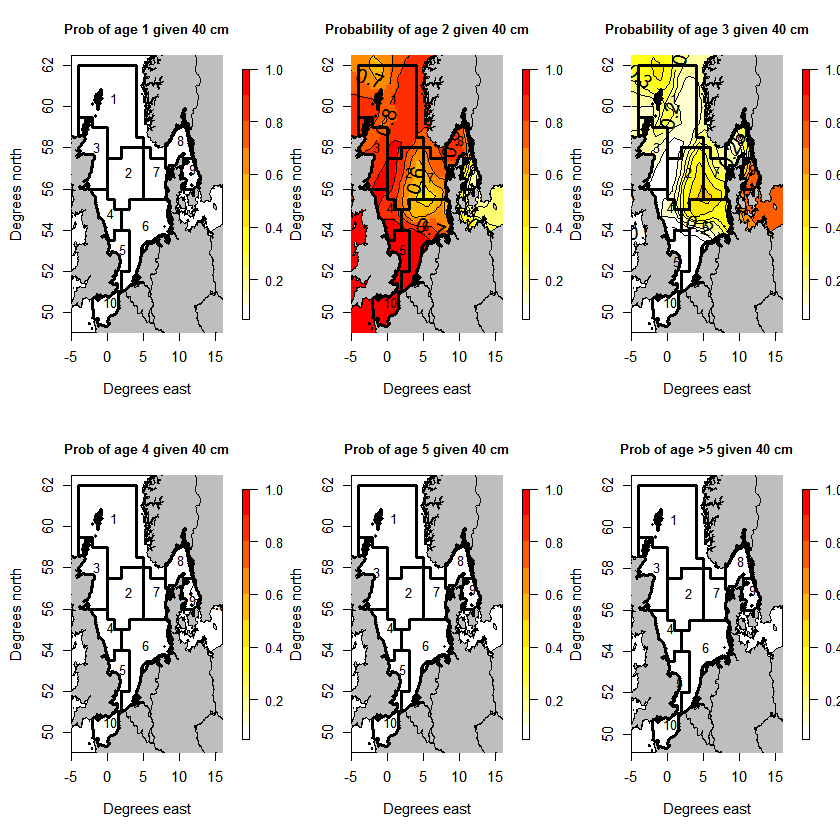
\includegraphics[scale=0.4]{Allcode40cm2015.png}
\caption{Estimated probability of age of a 40 cm long cod in the first quarter of year 2015. The probability of age three or older is approximately zero. The polygones marked 1 to 10 is the round fish areas (RFAs) where the ALK is assumed constant in the currently used estimators of the official CPUEs.}\label{fig:40cmCod2015}
\end{figure}

\subsection{Overview of the North Sea International Bottom Trawl Surveys}
\label{overview}
\indent The North Sea International Bottom Trawl Survey was formed in 1991, which is a combination of the International Young Herring Survey (IYHS) and eight national surveys in the North Sea, Skagerrak and Kattegat areas. These surveys began in the 1960's, and the 1970's and 1980's, respectively. The IYHS was developed with the aim of obtaining annual recruitment indices for the combined North Sea herring \emph{Clupea harengus} stock \citep{ICES2012}, but yielded valuable information on other fish species such as cod \emph{Gadus morhua} and haddock \emph{Melanogrammus aeglefinus}.\\
\indent The North Sea IBTS began with quarterly surveys providing information on seasonal distribution of stocks sampled, hydrography and the environment, which allows changes in fish stock to be monitored and abundance of all fish species (Table \ref{fishspecies}) to be determined. These quarterly surveys, however became difficult to sustain as countries experienced budget cuts making it impossible to maintain high levels of research vessel effort. As such, in 1997 countries carried out a survey only twice a year; a first quarter survey (January-February) and a third quarter survey (August-September). Table \ref{fishspecies} gives the common names (scientific names in parentheses) of the target species that are sampled during the quarterly North Sea International Bottom Trawl Surveys. The common names of the species in parentheses will be used in the rest of paper.\\

\begin{small}
\begin{table}[h!]
\centering
\setlength\tabcolsep{1.5pt} 
\captionsetup{font=small, width = 8.5cm}{
\caption{Species fished in the NS-IBTS from 1991-2017.}\label{fishspecies}}
\begin{tabular}{cccccccccc}
\hline \\
\multicolumn{2}{c}{} \\
Standard Pelagic               & Standard Roundfish & By-Catch Gadoid       \\[1.5ex]
%\cmidrule(lr{0.5em}){1-1} \cmidrule(lr{0.5em}){2-2}\cmidrule(lr{0.5em}){3-3} \\ [0.1ex]
\hline \\[0.1ex]
Herring (Clupea harengus) &  Cod (Gadus morhua)  & Pollock (Pollachius)      \\[1.5ex]
Sprat (Sprattus sprattus)   &Haddock (Melanogrammus aeglefinus) & Pouting (Trisopterus luscus) \\[1.5ex]
Mackerel (Scomber scombrus) & Norway Pout (Trisopterus esmarkii) & Trisopterus minutus (Poor Cod) \\[1.5ex]
 & Saithe (Pollachius virens)  & Blue Whiting (Micromesistius poutassou)   \\[1.5ex]
&Whiting (Merlangius merlangus)  & Hake (Merluccius merluccius)  \\[1.5ex]
& &  Ling (Molva molva) \\[1.5ex]
& &  Tusk (Brosme brosme) \\[0.5ex]
\hline
\end{tabular}
\end{table}
\end{small}

\indent Research vessels from seven nations in the first quarter (Q1) and six nations in the third quarter (Q3) are used for conducting surveys on all finfish species in the North Sea during January-February and July-August, respectively, between 1997-2017 (see Table \ref{countries} in appendix \ref{areasfishedappendix}). The sampling frame is defined by the ICES index or roundfish areas (RFA) as shown in Figure \ref{icesroufismap} numbered 1 to 10, and which we refer to as superstrata \citep{nottestad2015quantifying, fuller2011sampling}. These  roundfish areas were substratified into small strata defined by non-overlapping statistical rectangles of roughly $30 \times 30$ nautical miles ($1^{o} \  \mathrm{Longitude} \ \times  \  0.5^{o} \ \mathrm{Latitude}$), and were convenient to use for North Sea IBTS as they were already being used for fisheries management purposes. Most statistical rectangles contain a number of possible tows that are deemed free of obstructions, and vessels are free to choose any position in the rectangles as long as the hauls are separated by at least 10 nautical miles within and between rectangles. However, all countries select tows based on a semi-random approach from datababes of national safe tows or DATRAS or commercial fishing data, except Sweden who uses fixed stations and in some cases depth-stratified semi-random sampling design \citep{ICES2018}, and England who also uses fixed stations and only conduct surveys during the third quarter. In some rectangles, sampling may be further stratified due to significant changes in seabed depth which may, in turn, cause variations in the fish population. In particular, the North Sea IBTS herring, saithe and sprat data are weighted by depth strata in the statistical rectangle (see Table \ref{weightings11} in appendix \ref{secAp:weightings}). It is also a requirement that countries avoid clustering their stations between adjacent rectangles in order to reduce positive serial correlation, and thereby maximize survey precision.  The latest major reallocation of rectangles occurred in 1991, but since then the survey has tried to keep at least one vessel in every subarea in which it had fished in the most recent years. Minor reallocation of rectangles between Norway, Scotland and Germany was done in 2013. Each rectangle was  typically sampled twice by two different countries before 1997, but after that target coverage of two trawl hauls per rectangle per survey  was introduced because of national financial constraints \citep{ICES2015}. But in some rectangles in the Eastern English Channel, Southern North Sea and Central North Sea intensified sampling is carried out.\\
\indent The recommended standard trawling gear of the North Sea IBTS is the mulitpurpose chalut {\`a} Grande Ouverture Verticale (GOV) trawl \citep{ICES2012}, which has been used on all participating vessels since 1992, while different pelagic and bottom trawls suitable for fishing finfish species were used before 1992. Standardized trawling protocols were adopted with a towing speed of 4 knots but depending on vessel performance, tide and weather conditions the average towing speed can be at minimum 3.5 and maximum 4.5 knots. From 2000-2018 trawling is done during the daylight hours, which are considered 15 minutes before sunrise to 15 minutes  after sunset \citep{ICES2012}. After each trawl the total catch of the different species is weighed on board and biological parameters such as length for all fish species caught (to 0.1$\cm$ below for shellfish, to 0.5$\cm$ below for herring and sprat and to 1$\cm$ below for all other species) are collected. Where the numbers of individuals are too large for all of them  to be measured to obtain the length distribution, a representative subsample of 100 fish is selected. Otoliths are collected on board from a small fraction of all the target species from all  round fish areas (RFAs) (Figure \ref{icesroufismap}) to retrieve age reading. Table \ref{otolithsTable} in appendix \ref{sec:otolithappendix} gives the minimum sampling levels of otoliths for the target species.
%\indent The trawl tow locations are selected using a  semi-random approach with at least two primary sampling units (PSU) per stratum, where PSUs are standardized swept-area trawl hauls. Sampling locations for all countries are proposed in advance in order to increase the randomisation of sampling. These locations are based on a random selection on a random selection of valid tows with start and end position executed in the period 2000-2017. In the unusual event that no ``clear" tow exists the cruise leader, who select the haul positions, may select to undertake a ``blind" tow on unknown ground after checking the proposed trawl track for hazardous seadbed obstructions with acoustic methods. \\

%\clearpage
\begin{figure}[h!]
  \centering
 {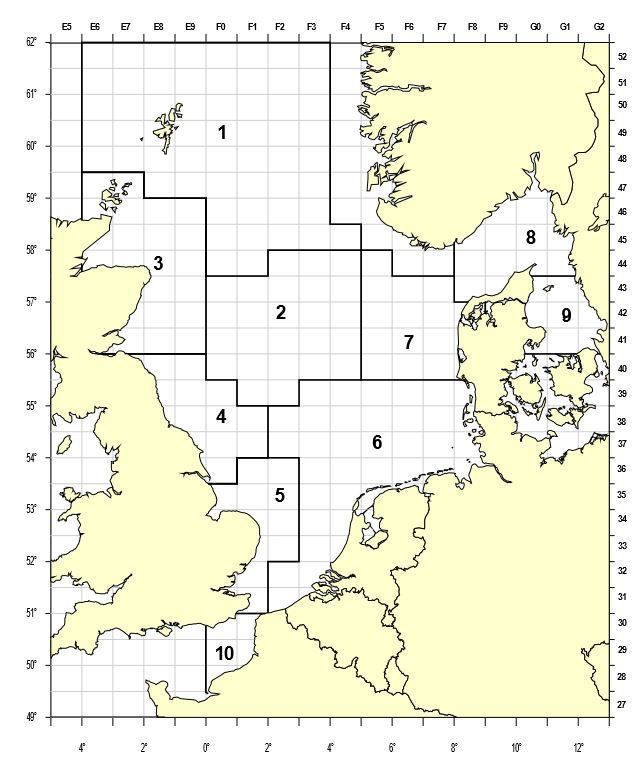
\includegraphics[width=11cm]{icesroundfishmap.jpg}}   
 \captionsetup{font= footnotesize, width=15cm}{
 \caption{Standard roundfish areas used for roundfish since 1980, for all standard species since 1991. Additional RFA 10 added in 2009. For example, the number 1 indicates ICES Index Area 1, and an ICES Statitical rectangle (ST) in IA 1 is 43F1 \citep{ICES2015}.}\label{icesroufismap}}
\end{figure}



%%%%\begin{small}
%%%\begin{table}[h!]
%%%\centering
%%%\setlength\tabcolsep{1.5pt} 
%%%\captionsetup{font=small, width = 10cm}{
%%%\caption{Age-length compositons and number at age-length key (ALK) in the first quarter of 2015.}\label{agelengthcomposition}}
%%%\begin{tabular}{ccccccccccccccccccc}
%%%\hline \\
%%%{\bf Age $(a)$} &&& \multicolumn{3}{c}{\bf cod} && \multicolumn{3}{c}{\bf saithe} \\[1.5ex]
%%% &&& Number   && Length ($l$ in cm)  && Number   && Length ($l$ in cm)      \\[1.5ex]
%%%%\cmidrule(lr{0.5em}){1-1} \cmidrule(lr{0.5em}){2-2}\cmidrule(lr{0.5em}){3-3} \\ [0.1ex]
%%%\cmidrule(lr{0.5em}){4-6} \cmidrule(lr{0.5em}){7-10}
%%%1   &&&  460  &&  9.0 - 38.0   &&  17    &&  13.0 - 21.0     \\[1.5ex]
%%%2   &&&  1191 &&  16.0 - 63.0  &&  5    &&  30.0 - 51.0  \\[1.5ex]
%%%3   &&&  676  &&  24.0 - 84.1  &&  55   &&  31.0 - 48.0  \\[1.5ex]
%%%4   &&&  284  &&  30.0 - 93.0  &&  90   &&  38.0 - 62.0  \\[1.5ex]
%%%5   &&&  101  &&  52.0 - 94.2  &&  146  &&  43.0 - 68.0  \\[1.5ex]
%%%6   &&&  63   &&  62.0 - 104.0 &&  115  &&  48.0 - 83.0  \\[1.5ex]
%%%7   &&&  12   &&  75 - 98      &&  57   &&  54.0 - 92.0 \\[0.5ex]
%%%8   &&&  1    &&   113         &&  57   &&  57.0 - 95.0 \\[0.5ex]
%%%9   &&&  -    &&  -            &&  11   &&  70.0 - 95.0 \\[0.5ex]
%%%10   &&&  -   &&  -            &&  12   &&  66.0 - 95.0 \\[0.5ex]
%%%11   &&&  -   &&  -            &&  8    &&  81.0 - 97.0 \\[0.5ex]
%%%12   &&&  -   &&  -            &&  3    &&  90.0 - 100.0 \\[0.5ex]
%%%13   &&&  -   &&  -            &&  4    &&  85.0 - 105.0 \\[0.5ex]
%%%14   &&&  -   &&  -            &&  5    &&  89.0 - 110.0 \\[0.5ex]
%%%15   &&&  -   &&  -            &&  6    &&  87.0 - 96.0 \\[0.5ex]
%%%16   &&&  -   &&  -            &&  1    &&   87 \\[0.5ex]
%%%\hline
%%%\end{tabular}
%%%\end{table}
%%
%%%\clearpage
%%%\begin{small}
%%%\begin{table}[h!]
%%%\caption{Summary of North Sea IBTS cod and caithe data for first quarter of 2015.}
%%%\begin{tabular}{llllll}
%%%\toprule
%%%\bf Data&\bf Description \\
%%%\midrule
%%%Trawl hauls  & Total of 387 trawl hauls (303 with age information of cod)  \\[0.5ex]
%%%Age &The age of cod varied between 1 to 8 years. \\[0.5ex]
%%%Length & Length information in cm of each cod varied between 8 to 112 cm\\[0.5ex]
%%%Date&Date of catch varied between 13.01.2015 to 19.02.2015 \\[0.5ex]
%%%Statistical rectangle & The stratum in  which at least two trawl hauls are made \\[0.5ex]
%%%Coordinates & Geographic coordinates of each trawl haul in a statistical rectangle \\[0.5ex]
%%%Duration of haul & Mean duration is 25.9 minutes, with 15  to 30 minutes as 90\% coverage interval. \\[0.5ex]
%%%Total count per age ($\mathrm{Total_{age}}$) & $3017_{1}$, $2629_{2}$, $1773_{3}$, $1051_{4}$, $460_{5}$, $194_{6}$, $58_{7}$ \\[0.5ex]
%%%Total count for all ages & 7605 cod in the first quarter of 2015. \\[0.5ex]
%%%\bottomrule
%%%\end{tabular}
%%%\label{tab:data2015}
%%%\end{table}
%%%\end{small}
%%
%%%\clearpage



%\begin{figure*}[h!]
%\centering
%\begin{tabular}{@{}ccc@{}}
%\subfloat[age-length distribution of cod]{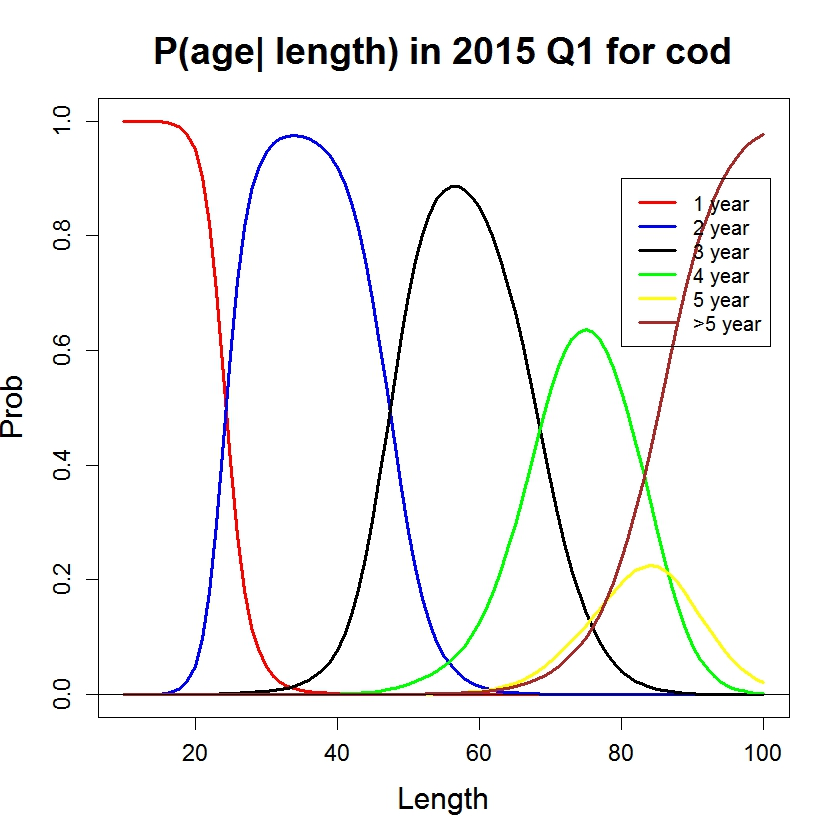
\includegraphics[width=0.5\textwidth]{cod2015Q1.jpeg}} & 
%\subfloat[age-length distribution of saithe]{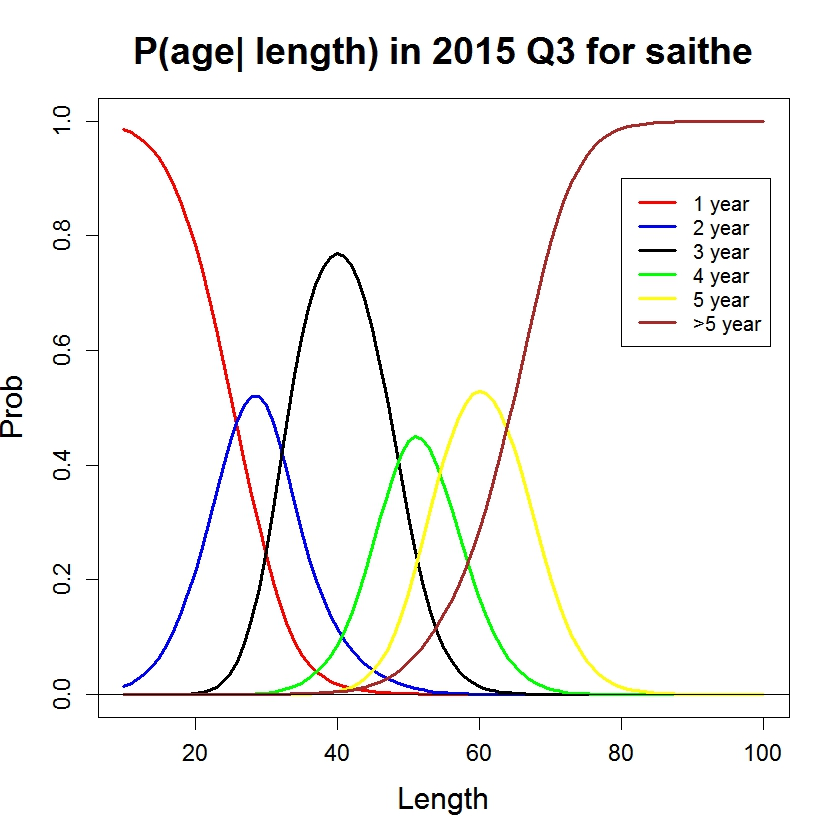
\includegraphics[width=0.5\textwidth]{saithe2015Q3.jpeg}} &
%\end{tabular}
%\caption[]{Predicted probabilities of age given length using the model described in (\ref{model}) for cod (left panel) and saithe (right panel) in Q1 and Q3, respectively for year 2015.}
%\label{fig:codandsaithe}
%\end{figure*}

%%%the probability of all trawl hauls containing missing age-length compositions of the {\bf two species} over an eight year period. Table \ref{probability} gives the probability of age given length of cod or saithe species from 2010-2017. In 2015, $89\%$ of the trawl hauls with at least one length observation of length $l$ of cod, had also an age observation for length $l$, and if we further condition that $l>50$ cm, at least $93\%$ of trawl hauls with at least one length observation of length $l$, had also an age observation for length $l$. {\bf For saithe....}. We also examine the distribution of trawl hauls with length and age information, and with only length information in the 10 round fish areas (Figure....). The  \\
%%
%%
%%%\clearpage
%%%\begin{figure}[h!]
%%%\centering
%%%\includegraphics[scale=0.4]{trawlHaulsGadusMorhua.pdf}
%%%\caption{Trawl hauls containing both age and length information (blue) and length information only (red)}\label{trawlHaulsGaduMorhua}
%%%\end{figure}
%%%
%%%
%%%\clearpage
%%%%\begin{small}
%%%\begin{table}[h!]
%%%\centering
%%%\setlength\tabcolsep{1.5pt} 
%%%\captionsetup{font=small, width = 10.5cm}{
%%%\caption{Probability of age given length data sampled from 2010-2017.}\label{probability}}
%%%\begin{tabular}{cccccccccccccccc}
%%%\hline \\
%%% {\bf Year} &&& \multicolumn{3}{c}{\bf cod}   \\[1.5ex]
%%%&&& $\mathrm{Pr}(a \ | \ l)$ && $\mathrm{Pr}(a \ | \ l > 50 \ \mathrm{cm})$    &&    \\[1.5ex]
%%%%\cmidrule(lr{0.5em}){1-1} \cmidrule(lr{0.5em}){2-2}\cmidrule(lr{0.5em}){3-3} \\ [0.1ex]
%%%%\hline \\[0.1ex]
%%% \cmidrule(lr{0.5em}){4-6} 
%%%2010   &&&  86.4 $\%$ && 83.2 $\%$     \\[1.5ex]
%%%2011   &&&  90.7 $\%$ && 92.4 $\%$  &&\\[1.5ex]
%%%2012   &&&  87.6 $\%$ && 92.0 $\%$  &&   \\[1.5ex]
%%%2013   &&&  88.1 $\%$ && 93.0 $\%$  &&     \\[1.5ex]
%%%2014   &&&  89.8 $\%$ && 93.7 $\%$  &&    \\[1.5ex]
%%%2015   &&&  89.3 $\%$ && 93.8 $\%$  &&    \\[1.5ex]
%%%2016   &&&  93.0 $\%$ && 93.7 $\%$  &&   \\[0.5ex]
%%%2017   &&&  95.5 $\%$ && 98.8 $\%$  &&  \\[0.5ex]
%%%\hline
%%%\end{tabular}
%%%\end{table}
%%%%\end{small}
%%%Probability of age given length data sampled from 2010-2017.

%\clearpage
%%\begin{small}
%\begin{table}[h!]
%\centering
%\setlength\tabcolsep{1.5pt} 
%\captionsetup{font=small, width = 11.5cm}{
%\caption{Fraction of trawl hauls with length information for cod and saithe that also had a corresponding age information for the period 2010-2017.}\label{probability}}
%\begin{tabular}{cccccccccccccccc}
%\hline \\
% {\bf Year} &&& \multicolumn{3}{c}{\bf cod} && \multicolumn{3}{c}{\bf saithe}  \\[1.5ex]
%  \cmidrule(lr{0.5em}){4-6} \cmidrule(lr{0.5em}){7-10}
%&&&all length groups && length groups $  > 50 \ \mathrm{cm}$    && all length groups && length groups $  > 50 \ \mathrm{cm}$    \\[1.5ex]
%%\cmidrule(lr{0.5em}){1-1} \cmidrule(lr{0.5em}){2-2}\cmidrule(lr{0.5em}){3-3} \\ [0.1ex]
%%\hline \\[0.1ex]
%2010   &&&  86.4 $\%$ && 83.2 $\%$  &&  86.4 $\%$ && 83.2 $\%$    \\[1.5ex]
%2011   &&&  90.7 $\%$ && 92.4 $\%$  &&  90.7 $\%$ && 92.4 $\%$ \\[1.5ex]
%2012   &&&  87.6 $\%$ && 92.0 $\%$  &&  87.6 $\%$ && 92.0 $\%$  \\[1.5ex]
%2013   &&&  88.1 $\%$ && 93.0 $\%$  &&  88.1 $\%$ && 93.0 $\%$   \\[1.5ex]
%2014   &&&  89.8 $\%$ && 93.7 $\%$  &&  89.8 $\%$ && 93.7 $\%$   \\[1.5ex]
%2015   &&&  89.3 $\%$ && 93.8 $\%$  &&  89.3 $\%$ && 93.8 $\%$   \\[1.5ex]
%2016   &&&  93.0 $\%$ && 93.7 $\%$  &&  93.0 $\%$ && 93.7 $\%$   \\[0.5ex]
%2017   &&&  95.5 $\%$ && 98.8 $\%$  &&  95.5 $\%$ && 98.8 $\%$   \\[0.5ex]
%\hline
%\end{tabular}
%\end{table}
%%\end{small}



%%%%\clearpage
%%%%\begin{small}
%%%\begin{table}[h!]
%%%\centering
%%%\setlength\tabcolsep{1.5pt} 
%%%\captionsetup{font=small, width = 9.5cm}{
%%%\caption{Fraction of trawl hauls with length information for cod and saithe that also had a corresponding age information for the period 2010-2017.}\label{probability}}
%%%\begin{tabular}{cccccccccccccccc}
%%%\hline \\
%%% {\bf Year} &&& \multicolumn{3}{c}{\bf cod} && \multicolumn{3}{c}{\bf saithe}  \\[1.5ex]
%%%&&& $\mathrm{Pr}(a \ | \ l)$ && $\mathrm{Pr}(a \ | \ l > 50 \ \mathrm{cm})$    && $\mathrm{Pr}(a \ | \ l)$ && $\mathrm{Pr}(a \ | \ l > 50 \ \mathrm{cm})$    \\[1.5ex]
%%%%\cmidrule(lr{0.5em}){1-1} \cmidrule(lr{0.5em}){2-2}\cmidrule(lr{0.5em}){3-3} \\ [0.1ex]
%%%%\hline \\[0.1ex]
%%% \cmidrule(lr{0.5em}){4-6} \cmidrule(lr{0.5em}){7-10}
%%%2010   &&&  86.4 $\%$ && 83.2 $\%$  &&  86.4 $\%$ && 83.2 $\%$    \\[1.5ex]
%%%2011   &&&  90.7 $\%$ && 92.4 $\%$  &&  90.7 $\%$ && 92.4 $\%$ \\[1.5ex]
%%%2012   &&&  87.6 $\%$ && 92.0 $\%$  &&  87.6 $\%$ && 92.0 $\%$  \\[1.5ex]
%%%2013   &&&  88.1 $\%$ && 93.0 $\%$  &&  88.1 $\%$ && 93.0 $\%$   \\[1.5ex]
%%%2014   &&&  89.8 $\%$ && 93.7 $\%$  &&  89.8 $\%$ && 93.7 $\%$   \\[1.5ex]
%%%2015   &&&  89.3 $\%$ && 93.8 $\%$  &&  89.3 $\%$ && 93.8 $\%$   \\[1.5ex]
%%%2016   &&&  93.0 $\%$ && 93.7 $\%$  &&  93.0 $\%$ && 93.7 $\%$   \\[0.5ex]
%%%2017   &&&  95.5 $\%$ && 98.8 $\%$  &&  95.5 $\%$ && 98.8 $\%$   \\[0.5ex]
%%%\hline
%%%\end{tabular}
%%%\end{table}
%%%%\end{small}
%%
%%%%\begin{small}
%%%\begin{table}[h!]
%%%\centering
%%%\setlength\tabcolsep{1.5pt} 
%%%\captionsetup{font=small, width = 8.5cm}{
%%%\caption{Age-length compositons of cod and total catch in all years.}\label{agelengthcomposition}}
%%%\begin{tabular}{cccccccccccc}
%%%\hline \\
%%%Age $(a)$ &&& Total  && Number measured && Length ($l$ in cm)     \\[1.5ex]
%%%%\cmidrule(lr{0.5em}){1-1} \cmidrule(lr{0.5em}){2-2}\cmidrule(lr{0.5em}){3-3} \\ [0.1ex]
%%%\hline \\[0.1ex]
%%%1   &&&  3017 && 2413 && 8.0 - 42.0    \\[1.5ex]
%%%2   &&&  2629 && 2087  &&  16.0 - 63.0 \\[1.5ex]
%%%3   &&& 1773  && 1310 && 24.0 - 83.30  \\[1.5ex]
%%%4   &&&  1051 && 723 &&  30.0 - 93.0  \\[1.5ex]
%%%5   &&&  460  && 322  && 49.0 - 111.0  \\[1.5ex]
%%%6   &&&  194 && 135  &&  57.0 - 105.0 \\[1.5ex]
%%%7   &&&  58 && 43 && 60.0 - 112.0 \\[0.5ex]
%%%\hline
%%%\end{tabular}
%%%\end{table}
%%
%%
%%
%%%\clearpage
%%%%\begin{small}
%%%\begin{table}[h!]
%%%\centering
%%%\setlength\tabcolsep{1.5pt} 
%%%\captionsetup{font=small, width = 8.5cm}{
%%%\caption{Age-length compositons of cod and total catch in the first quarter of 2015.}\label{agelengthcomposition}}
%%%\begin{tabular}{cccccccccccc}
%%%\hline \\
%%%Age $(a)$ &&& NoAtALK   && Length ($l$ in cm)     \\[1.5ex]
%%%%\cmidrule(lr{0.5em}){1-1} \cmidrule(lr{0.5em}){2-2}\cmidrule(lr{0.5em}){3-3} \\ [0.1ex]
%%%\hline \\[0.1ex]
%%%1   &&&  460  &&  9.0 - 38.0    \\[1.5ex]
%%%2   &&&  1191 &&  16.0 - 63.0 \\[1.5ex]
%%%3   &&&  676  &&  24.0 - 84.1  \\[1.5ex]
%%%4   &&&  284  &&  30.0 - 93.0  \\[1.5ex]
%%%5   &&&  101  &&  52.0 - 94.2  \\[1.5ex]
%%%6   &&&  63   &&  62.0 - 104.0 \\[1.5ex]
%%%7   &&&  12   &&  75 - 98 \\[0.5ex]
%%%8   &&&  1    &&   113\\[0.5ex]
%%%\hline
%%%\end{tabular}
%%%\end{table}
%%%
%%%
%%%
%%%%\begin{small}
%%%\begin{table}[h!]
%%%\centering
%%%\setlength\tabcolsep{1.5pt} 
%%%\captionsetup{font=small, width = 8.5cm}{
%%%\caption{Age-length compositons of cod and total catch in all years in the first quarter Q1.}\label{agelengthcomposition}}
%%%\begin{tabular}{cccccccccccc}
%%%\hline \\
%%%Age $(a)$ &&& NoAtALK   && Length ($l$ in cm)     \\[1.5ex]
%%%%\cmidrule(lr{0.5em}){1-1} \cmidrule(lr{0.5em}){2-2}\cmidrule(lr{0.5em}){3-3} \\ [0.1ex]
%%%\hline \\[0.1ex]
%%%1   &&&  1423  &&  8.0 - 38.0    \\[1.5ex]
%%%2   &&&  1561 &&  16.0 - 63.0 \\[1.5ex]
%%%3   &&&  1099  &&  24.0 - 84.1  \\[1.5ex]
%%%4   &&&  665  &&  30.0 - 93.0  \\[1.5ex]
%%%5   &&&  293   &&  51.0 - 94.2  \\[1.5ex]
%%%6   &&&  128   &&  57 - 105.0 \\[1.5ex]
%%%7   &&&  34   &&  66 - 112 \\[0.5ex]
%%%8   &&&  9    &&   60 - 113\\[0.5ex]
%%%\hline
%%%\end{tabular}
%%%\end{table}
%%
%%%
%%%\clearpage
%%%\begin{figure}[h!]
%%%  \centering
%%% {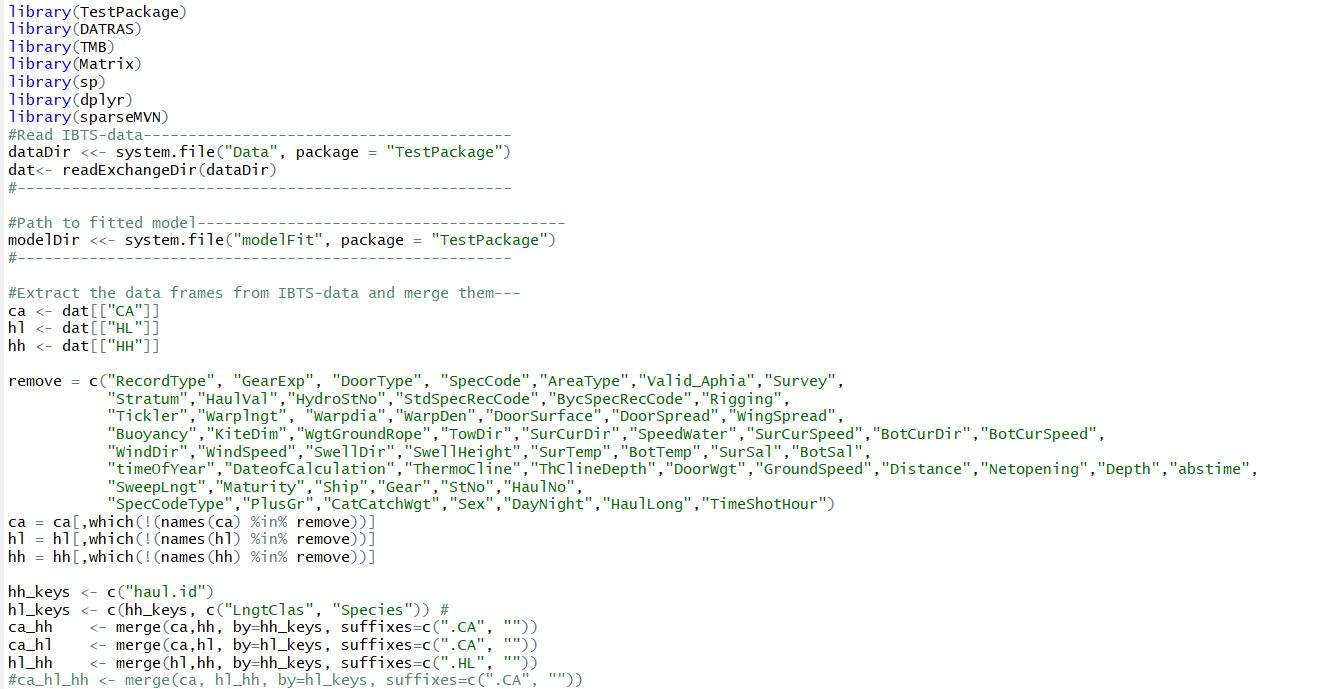
\includegraphics[width=19cm]{codetest.jpg}}   
%%% \captionsetup{font= footnotesize, width=20cm}{
%%% \caption{}\label{1254}}
%%%\end{figure}
%%%
%%
%%
%%%\clearpage
%%%\end{small}
%%%In 2017 for cod,  95.5% of every trawl haul with at least one length observation of length L, had also an age observation of length L.
%%%If we further condition on that L>50, then 98.8% of every trawl haul with at least one length observation of length L, had also an age observation of length L.
%%%
%%%For the other years we have in the same order:
%%
%%%[1] "Year  2010 :  86.4 %,  83.2 %"
%%%[1] "Year  2011 :  90.7 %,  92.4 %"
%%%[1] "Year  2012 :  87.6 %,  92 %"
%%%[1] "Year  2013 :  88.1 %,  93 %"
%%%[1] "Year  2014 :  89.8 %,  93.7 %"
%%%[1] "Year  2015 :  89.3 %,  93.8 %"
%%%[1] "Year  2016 :  93 %,  93.7 %"
%%%[1] "Year  2017 :  95.5 %,  98.8 %"

\section{\large METHODS}
\label{sec:methods}
This section gives the estimators of abundance indices. The estimators are haul time-based and utilizes an ALK approach. We consider the ALK approach used in DATRAS and we propose two ALK estimators. The ALK used in DATRAS for computing abundance indices does not account explicitly for the spatial distribution in the age-length composition, which may be different and would result in a biased ALK. This difference may be caused either by variation in length-at-age distributions or by variations in the relative abundance of age classes, that is age-at-length distributions \citep{gerritsen2006simple}.  To account for the spatial distribution we propose a design-based ALK estimator that is haul dependent (Section \ref{sec:haulestimator}) and a model-based ALK estimator (\ref{sec:spatialModelALK}).

\subsection{Catch per unit effort}
\label{sec:cpueestimators}
In this section we define an estimate of the mean catch per unit effort (mCPUE), which is the index used in assessment. For a given species of interest, define $n_{h,l}$ to be the number of fish with length $l$ caught by the $h$th trawl haul. Define the CPUE for a given trawl $h$ of fish at length $l$ to be 

\begin{equation}\label{eq:cpueHaul}
\mathrm{CPUE}_{h,l} =\frac{n_{h,l}}{d_h},
\end{equation}
were $d_h$ is the duration of the trawl in hours. The CPUE per age class is further defined as
\begin{equation}\label{eq:cpueALK}
\mathrm{CPUE}_{h,a} =\sum_{l \in {\bf L}}\mathrm{CPUE}_{h, l} \times ALK_{a,l,h},
\end{equation}
where ${\bf L}$ is the set of all length classes and $ALK_{a,l,h}$ is an age length key which represents the estimated proportion of fish with age $a$ in $l$th length class in haul $h$. The mCPUE in a statistical rectangle is further defined as the average of the CPUE for each trawl haul in the rectangle:
\begin{equation}\label{eq:cpueRec}
\mathrm{mCPUE}_{s,a} =\sum_{h \in H_{s}}\frac{\mathrm{CPUE}_{h,a}}{|H_{s}|}.
\end{equation}
Here $H_{s}$ represents the set of trawl hauls taken in statistical rectangle $s$, and $|H_{s}|$ is the number of hauls taken in the rectangle. The mCPUE in $p$th RFA is further defined as
\begin{equation}\label{eq:cpueRFA}
\mathrm{mCPUE}_{p,a} = \sum_{s \in S_{p}} \frac{\mathrm{mCPUE}_{s,a}}{|S_{p}|} \omega_s,
\end{equation}
where $S_{p}$ is the set of all statistical rectangles in $p$th RFA, $|S_{p}|$ is the number of statistical rectangles in $p$th RFA, and $\omega_s$ is a weight variable for each statistical rectangle. The weight variable $\omega_i$ is varies with species. For some species it equals 1 (e.g. gadus morhua), and for other species it is the proportion of the statistical rectangle which has depth between 10 to 200 meters (e.g. pollachius virens).  The index for abundance at age in the whole study area, $mCPUE_{N,a} $, is defined by
\begin{equation}
mCPUE_{N,a} = \frac{\sum_{p\in {\bf P}} A_{p}  \mathrm{mCPUE}_{p,a}}{A_{\text{total}}}.
\label{abundanceestimatornorthsea}
\end{equation}
Here ${\bf P}$ is the set of round fish areas, $A_p$ is the area of round fish area $p$, and $A_{\text{total}} = \sum_{p\in {\bf P}} A_{p}$.

 
%\noindent For known variances of  $\mathrm{mCPUE}_{p,a} $, the variance of the mean abundance at age across supuerstrata,  $mCPUE_{N,a}$, can be computed directly as 
%\begin{equation}
%\mathrm{Var} \left(mCPUE_{N,a}\right) =  \frac{\sum_{p=1}^{P} {A}_{p}^{2}  \mathrm{Var}\left(\mathrm{mCPUE}_{p,a} %\right)}{\displaystyle{A}_{N}^{2}}.
%\end{equation}

%{\bf a combined ratio estimator with suitable variance estimator may be more appropriate than this current separate ratio estimator for the north sea}
%$N_{\text{RFA}}^{(i)}$
%computed as the mean abundance at age across superstrata, that is, the ratio 
%of estimated 
%using combined ratio estimator 
%\emph{An estimator for catch at age in the North Sea is needed, and variance estimator}

%\indent The cpue per age class is further defined as
%\begin{equation}\label{eq:cpueALK}
%\mathrm{CPUE}_{h,a} =\sum_{l \in {\bf L}}\mathrm{CPUE}_{h,l} \times ALK_{a,l,h},
%\end{equation}
%where $ALK_{a,l,h}$ is an age length key which represents the estimated proportion of fish with age $a$ in $l$th length class in haul $h$, and ${\bf L}$ is the set of all length classes. The mean CPUE per age in the statistical rectangles and roundfish areas are defined as (\ref{eq:cpueRec}) and (\ref{eq:cpueRFA}) with $\mathrm{CPUE}_{(\cdot),l}$ substituted by $\mathrm{CPUE}_{(\cdot),a, l}$.  \\




\subsection{ALK Estimators}

Three ALK estimators are presented in this section. The first is the DATRAS ALK estimator and two estimators that consider spatial variation in the data; a Haul based ALK estimator and a Model based ALK estimator.

\subsubsection{DATRAS ALK Estimator }
\label{sec:datrasalkestimator}
Let $ALK^{\text{D}}$ be the ALK used in DATRAS, which is currently used for producing offical CPUE per age estimates. This is an aggregation of individual samples from a haul combined over a larger area, in this a round fish area (RFA). The $ALK^{\text{D}}_{a,l,h}$ is defined as the proportion of observed fish with age $a$ in length class $l$ in the RFA. If there are no observed fish in length class $l$ in the RFA, ages from length classes close to $l$ is used. The details of the procedure for borrowing strength from neighbouring length classes are given in appendix \ref{secAp:DATRASBorrow}. The underlying assumption of this  $ALK^{\text{D}}$ approach is that age-length compositions are homogeneous within the RFAs. This is a rather strong assumption, and any violation have an unknown impact on the estimates of abundance indices. In fact, \citet{kimura1977statistical} showed that the application of an age-length key  to a population where the age composition differs from that of the population from which the age-length key was drawn will give bias results. Because the age-length key may be haul dependent we propose an ALK method that is based on trawl hauls, which we denote by $\mathrm{ALK}^{H}$. 

\subsubsection{Haul Dependent ALK Estimator}
\label{sec:haulestimator}
We define a haul dependent ALK  by  $ALK^{H}$. The $ALK^{H}_{a,l^*,h}$ is defined as the average proportion of observed fish with age $a$ in a pooled length class $l^*$ in haul $h$. We use pooled length classes for this estimate since there are typically few observed length classes in a single haul. We define a pooled length class to consist of five length classes, the first pooled length class consist of the five smallest length classes and so on.  If there are no observed ages of fish in a pooled length class $l^*$ in the haul, ages from the same pooled length class in the haul closest in air distance from the $h$th haul is used. If there are no observed fish within the pooled length class in the closes haul, the next closes haul is used and so on.  The details of borrowing strength from length classes in hauls closest in space is given in appendix \ref{secAp:oursBorrow}. 

\subsubsection{Spatial Model-Based ALK Estimator}
\label{sec:spatialModelALK}
In this section we introduce a spatial model based ALK. Including such a model enables us to utilize smooth structures in the distribution of age given length. It further enables us to utilize spatial latent effects and possible haul based variation. Spatial model-based approach of age-lengths has been widely used in fisheries assessment \citep{berg2012spatial, kvist2000using, rindorf2001analyses}. \\
\indent Let the response variable of the age group of a fish be $a = M,...,A$ where $M$ is the youngest age and $A$ is the oldest age, which is typically defined as a "plus group". Suppose $y(l,{\bf s},h)$ is the age  of a fish with length $l$, caught at location ${\bf s}$ by trawl haul $h$, then the the probability of age $a$ in a given year and quarter is given by:
\begin{align}
\pi_a(y(l,{\bf s},h)) =
\begin{cases}
\frac{\exp(\mu_a)}{1+ \sum_{i = M}^{A-1} \exp(\mu_a)} ,& a<A \\
\frac{1}{1+ \sum_{i = M}^{A-1} \exp(\mu_a)},& a=A.
\end{cases},
\label{model}
\end{align}
where 
\begin{align}\label{eq:linearPred}
\mu_a(l,{\bf s},h) = f_a(l)  + \gamma_a({\bf s}) \big(1+ \nu_a(h)\big).
\end{align}
Here $ f_a^l(l)$ is a continuous function of length, $\pmb{\gamma}$ is a mean zero Gaussian spatial random field with Mat\'{e}rn covariance function, and $\pmb{\nu}$ is an independent identically distributed Gaussian random haul effect. The spatial random field is intended to capture any spatial variation in the ALK. The haul random effect is intended to capture any haul variations, for example, a haul may by chance hit a school of fish of a certain age.\\  
\indent The continous function $f_a^l(l)$ is modelled with usage of P-splines, \citep{wood2017generalized}. This is acheved by including the spline regression coefficients as Gausian random effect. The precision matrix for the spline regression coefficients is constructed such that wigglyness in the spline is penalized, see \citet[page 239]{wood2017generalized} for details. The R package mgcv \citep{wood2015package} is used for extracting the precision matrix needed for the spline regression coefficients.

\indent We assume that the spatially Gaussian random field in (\ref{eq:linearPred}), $\pmb{\gamma}$, follows a stationary Mat\'{e}rn covariance structure:
\begin{align}\label{eq:matern}
 \text{Cov}(\gamma(\mathbf{s}_1),\gamma(\mathbf{s}_2)) = \frac{\sigma^2_{\gamma}}{2^{\nu-1}\Gamma(\nu)}(\kappa_{\gamma}||\mathbf{s}_1 -\mathbf{s}_2||)^{\nu}K_{\nu}(\kappa_{\gamma}||\mathbf{s}_1-\mathbf{s}_2||),
\end{align}
where $\sigma^2_{\gamma}$ is the marginal variance, $||\cdot||$ is the Euclidean distance measure in kilometres, $\nu$ is a smoothing parameter, $\kappa_{\gamma}$ is a spatial scale parameter and $K_{\nu}(\cdot)$ is the modified Bessel function of the second kind with $\nu = 1$. The spatial range parameter and marginal variances in the spatial fields are assumed to be equal across ages. The spatial field is estimated with the stochastic partial differential equation (SPDE) procedure described in \citet{lindgren2011explicit}. The theory behind the SPDE procedure is based on that the precision matrix of a spatial field with Mat\'{e}rn  covariance function can be approximated by a sparse matrix on a grid covering the area of interest. Such a grid and sparse precision matrix are constructed with use of the R-INLA package \citep{rue2009approximate}.\\
\indent For each trawl haul, an ALK is obtained by maximizing the likelihood of the model in (\ref{model}). The maximum likelihood estimate of ${\mu}_{a}$  is obtained using the R-package TMB \citep{kristensen2015tmb} combined with the optimizing function \textit{nlminb} in R. Advantages of using TMB in this application is that it utilizes sparse structures in the latent fields, it Laplace approximate the latent fields, and uses automatic derivation. A laptop with  processor intel(R) Core(TM) i5-6300 CPU @ 2,40 GHz, used approximately 2 minutes to estimate the model. \\ 


In \citep{berg2012spatial} a Continuous ratio logit (CRL) models were applied for estimation a spatial ALK. \textit{Olav: Suggest we change to the same, should not make much of a difference. Had not have time to look at this yet, but it seems straight forward. And they refer to a book which seems to argue for their suggestion.} % We consider Logits \citep{dyke1952analysis,agresti2003categorical}, which is a type of model for categorical response data (such as age groups). Such a , which have been previously used for modelling ALKs with uncertainty \citep{gerritsen2006simple}.
%\indent Fish of a certain age might have a larger mean length in one area than another as a consequence of differential growth rates or size-specific migration. This is also the case for different species as can be seen in  \ref{fig:codandsaithe} which shows the age-length distributions of cod (left panel) and saithe (right panel). ({\bf is the plot below a prediction of the whole north sea or specific areas of the North sea?})

%\begin{figure*}[h!]
%\centering
%\begin{tabular}{@{}ccc@{}}
%\subfloat[age-length distribution of cod%{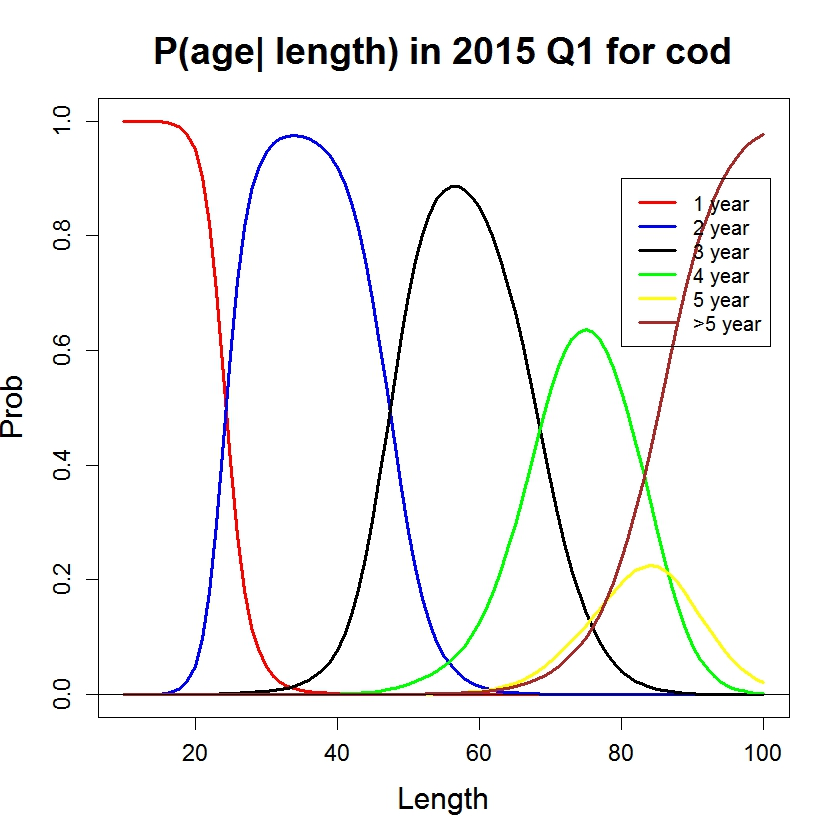
\includegraphics[width=0.5\textwidth]{cod2015Q1.jpeg}} & 
%\subfloat[age-length distribution of saithe]{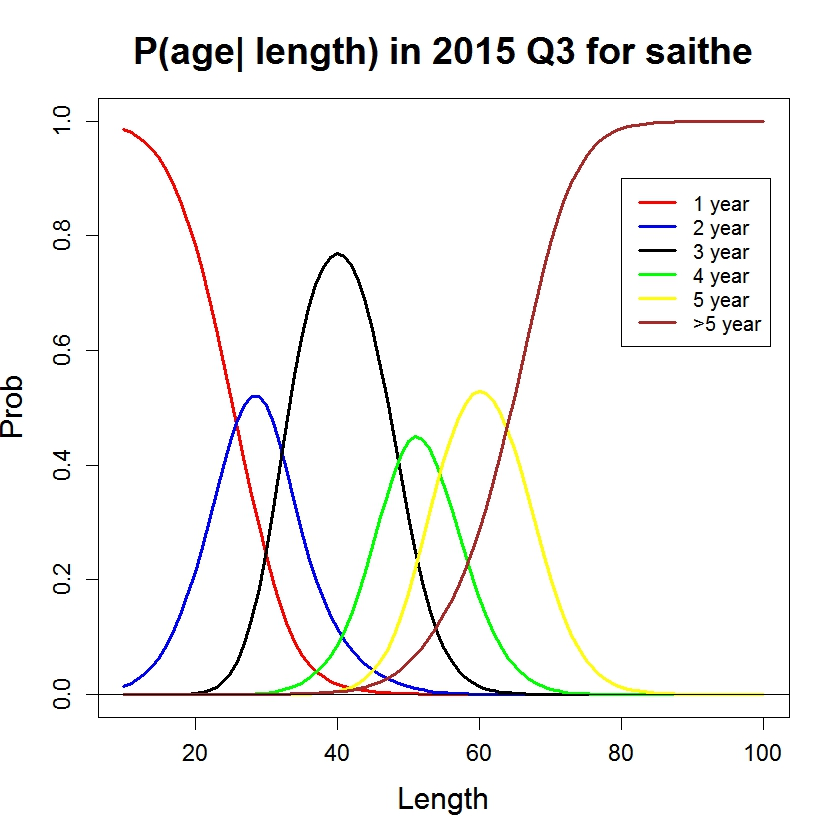
\includegraphics[width=0.5\textwidth]{saithe2015Q3.jpeg}} &
%\end{tabular}
%\caption[]{Predicted probabilities of age given length using the model described in (\ref{model}) for cod (left panel) and saithe (right panel) in Q1 and Q3, respectively for year 2015.}
%\label{fig:codandsaithe}
%\end{figure*}



%\begin{enumerate}
%\item Sample $m$ observations randomly with replacement from ${\bf x}$ to obtain a bootstrap data set, denoted by ${\bf {x}^{*}$.
%\item Calculate the bootstrap version of the statistic of interest, ${\theta}^{*} = \hat{\theta}({\bf {x}^{*}})$.
%\item Repeat steps 1 and 2 a large number of times, say $B$, to obtain an estimate of the bootstrap distribution
%\item calculate the average of the bootstrapped statistics, $\sum_{b=1}^{B} {{\theta}^{*}}_{(b)}/B$ 
%\item compute the variance of the estimator $\hat{\theta}({\bf x})$ through the variance of the set ${{\theta}^{*}}_{(b)}, \ b = 1,2,...,B,$ given by 
%
%$$ \frac{ \sum_{b=1}^{B} {\left({{\theta}^{*}}_{(b)} - {{\theta}^{*}}_{(\cdot)} \right)}^{2}  }{(B-1)}  $$
%
%where ${{\theta}^{*}}_{(\cdot)} = \sum_{b=1}^{B} {{\theta}^{*}}_{(b)}/B $ \citep[see][]{carpenter2000bootstrap}.
%\end{enumerate}
%\subsubsection{Stratified bootstrap procedure}
%\label{stratboot}


%Statistical inference and the theory of Gaussian fields
%Inferences using SPMs can be of two sorts depending on whether one knows where to look in advance. With an anatomically constrained hypothesis, about effects in a particular brain region, the uncorrected p value associated with the height or extent of that region in the SPM can be used to test the hypothesis. With an anatomically open hypothesis (i.e. a null hypothesis that there is no effect anywhere in a specified volume of the brain) a correction for multiple dependent comparisons is necessary. The theory of Gaussian random fields provides a way of correcting the p-value that takes into account the fact that neighboring voxels are not independent by virtue of continuity in the original data. Provided the data are sufficiently smooth the GRF correction is less severe (i.e. is more sensitive) than a Bonferroni correction for the number of voxels. As noted above GRF theory deals with the multiple comparisons problem in the context of continuous, spatially extended statistical fields, in a way that is analogous to the Bonferroni procedure for families of discrete statistical tests. There are many ways to appreciate the difference between GRF and Bonferroni corrections. Perhaps the most intuitive is to consider the fundamental difference between a SPM and a collection of discrete T values. When declaring a connected volume or region of the SPM to be significant, we refer collectively to all the voxels that comprise that volume. The false positive rate is expressed in terms of connected [excursion] sets of voxels above some threshold, under the null hypothesis of no activation. This is not the expected number of false positive voxels. One false positive volume may contain hundreds of voxels, if the SPM is very smooth. A Bonferroni correction would control the expected number of false positive voxels, whereas GRF theory controls the expected number of false positive regions. Because a false positive region can contain many voxels the corrected threshold under a GRF correction is much lower, rendering it much more sensitive. In fact the number of voxels in a region is somewhat irrelevant because it is a function of smoothness. The GRF correction discounts voxel size by expressing the search volume in terms of smoothness or resolution elements (Resels). See Figure 6. This intuitive perspective is expressed formally in terms of differential topology using the Euler characteristic (Worsley et al 1992). At high thresholds the Euler characteristic corresponds to the number of regions exceeding the threshold. \\
%There are only two assumptions underlying the use of the GRF correction: (i) The error fields (but not necessarily the data) are a reasonable lattice approximation to an underlying random field with a multivariate Gaussian distribution. (ii) These fields are continuous, with a twice-differentiable autocorrelation function. A common misconception is that the autocorrelation function has to be Gaussian. It does not. The only way in which these assumptions can be violated is if; (i) the data are not smoothed (with or without sub-sampling of the data to preserve resolution), violating the reasonable lattice assumption or (ii) the statistical model is mis-specified so that the errors are not normally distributed. Early formulations of the GRF correction were based on the assumption that the spatial correlation structure was wide-sense stationary. This assumption can now be relaxed due to a revision of the way in which the smoothness estimator enters the correction procedure (Kiebel et al 1999). In other words, the corrections retain their validity, even if the smoothness varies from voxel to voxel.


\subsection{Uncertainty estimation}
\label{sec:uncertaintyestimation}
We use nonparametric bootstrapping to estimate the uncertainty of age of estimated CPUEs. Nonparametric resampling allows us to estimate the sampling distribution of the catch per unit effort empirically without making assumptions concerning the data. The percentile method is used to estimate $95\%$ confidence intervals of the estimated CPUEs,. To obtain sufficiently accurate $95\%$ bootstrap percentile confidence intervals, the number of bootstrap samples should  be on the order of 1000 or more \citep[see][]{carpenter2000bootstrap}. 
\indent We start with the bootstrap procedure proposed by \emph{DATRAS} \citep{ICES2013} for this complex survey data. To construct the $b$th replicate, take a simple random sample with replacement of $N_{\text{p}}$ trawl hauls from the original data in the combined strata in the round fish area (RFA) and placing it into the relevant statistical rectangle (stratum $s$); repeat independently across strata; estimate the parameter of interest, for example in (\ref{eq:cpueHaul}); assuming $O_i$ is the number of age observations from the $i$th length class in the RFA, sample with replacement $O_i$ of these observations, and, if there is only one observed age in that length class sample either that fish or one which is closest in "length class distance"; estimate the parameters of interest: ALK defined in (\ref{sec:datrasalkestimator}) and catch per unit effort per age class in (\ref{eq:cpueALK}), followed by the parameters defined for each stratum $s$ and superstratum $p$ in (\ref{eq:cpueRec}), and (\ref{eq:cpueRFA}) and (\ref{eq:ageIndex}), respectively; repeat $B$ times; and estimate the variance using 
\begin{equation}
 \frac{ \sum_{b=1}^{B} {\left({{\theta}^{*}}_{(b)} - {{\theta}^{*}}_{(\cdot)} \right)}^{2}  }{(B-1)}  
 \label{eq:varianceforboot}
\end{equation}
where ${{\theta}^{*}}_{(b)} $ is the bootstrap version of the statistic of interest. An example in this case is the mean catch per unit effort for age $a$ in superstratum $p$ given in (\ref{eq:ageIndex}); and ${{\theta}^{*}}_{(\cdot)} $ is the average of the bootstrapped statistics, that is, $ \sum_{b=1}^{B} {{\theta}^{*}}_{(b)}/B$. This bootstrap procedure does not preserve the location of the trawl hauls, that is, stratification of trawl hauls is ignored, hence it is a simple nonparametric resampling procedure. Given the complex nature of the survey, this simple nonparametric resampling is not suitable \citep{kolenikov2010resampling}. The procedure is also based on the assumption that age-length structures are the same across strata within a round fish area  \\
\indent We propose the \emph{naive} bootstrap procedure \citep{kolenikov2010resampling} for complex survey data as an alternative to the DATRAS procedure for the ALK approach given in (\ref{sec:datrasalkestimator}). To construct the $b$th replicate, take a simple random sample with replacement  $N_{\text{s}}$ trawl hauls from the original data in stratum $s$; repeat independently across strata; estimate the parameter of interest in (\ref{eq:cpueHaul}); sample the age observations  $O_i$  as is done by the DATRAS procedure and estimate the ALK defined in (\ref{sec:datrasalkestimator}) followed by the parameters of interest in (\ref{eq:cpueALK}), (\ref{eq:cpueRec}), (\ref{eq:cpueRFA}) and (\ref{eq:ageIndex}); repeat $B$ times; and estimate the variance using (\ref{eq:varianceforboot}). \\
\indent For our proposed ALK estimators in (\ref{sec:haulestimator}) and (\ref{sec:spatialModelALK}) we consider two bootstrap procedures. The first procedure, which we call the \emph{stratified} bootstrap procedure is similar to the naive bootstrap described above. To construct the $b$th replicate, take a simple random sample with replacement  $N_{\text{s}}$ trawl hauls from the original data in stratum $s$, and if there is only one trawl haul in stratum $s$ sample either that trawl haul or one closest in ''air distance"; repeat independently across strata; estimate the parameter of interest in (\ref{eq:cpueHaul}); the ALKs defined in (\ref{sec:haulestimator}) and \ref{sec:spatialModelALK}) are also estimated from this sample; estimate further the parameters of interest in (\ref{eq:cpueALK}), (\ref{eq:cpueRec}), (\ref{eq:cpueRFA}) and (\ref{eq:ageIndex}) and estimate the variance using (\ref{eq:varianceforboot}). The stratified bootstrap procedure accounts for the variation within stratum $s$ but does not account for the variation between strata. \\
\indent  The second procedure is a \emph{hierarchical} bootstrap procedure by \citep{ren2010nonparametric}. The current data structure of IBTS is hierarchical in nature and such data types often includes multiple sources of variation. As such such, it would be important to take careful account of the multiple sources of variation as we are interested in abundance-at-age in North sea, which is computed based estimates obtained from strata and superstrata. The North Sea IBTS data has three level; haul, statistical rectangle (stratum $s$) and round fish area (superstratum $p$) but since an estimator for catch-at-age is provided for superstratum $p$ we use a two-level hierarchical sampling strategy (hauls and statistical rectangle) for estimating uncertainty at the superstratum level, and a combined ratio estimator approach, described in ......., is used for estimating the uncertainty for the whole North Sea area. To construct the $b$th replicate assume there are $S$ statistical rectangles (strata) in the $p$th RFA, and $H_{s}$ trawl hauls in the $s$th statistical rectangle. At the first stage a random integer $S^{*}$ from $\left\{1,2,..., S \right\}$ is chosen. At the second stage, we select $H_{s^{*}}$ random integer .....({\bf both statistical rectangle and haul and sample 1 to n inclusive is chosen to be in the sample)}... \\


{\bf explain how confidence intervals are formed (percentile method)}

\subsection{Optimizing Sampling Effort}
\label{sec:optimizationsampling}

%The North sea IBTS is carried twice a year: quarter 1 (January -February) and quarter 3 (July-September). We examined the sampling effort carried out over a five year period for IBTS for both quarters. From 2013 to 2018, on average there were 368 valid trawl hauls taken over an average period of 43 ship days in the first quarter between 6 nations, and 346 valid trawl hauls taken over an average of... ship days in third quarter between 7 nations. The number of otolith sampling per species per varies per length group and by nation. Some nations, for example......have been sampling otoliths per round fish area according the ICES guidelines \citep{ICES2006} during the years 2013-2017, while other nations such as Norway, UK Scotland and Netherlands have adopted a per-haul basis of sampling otoliths (see Table \ref{otolithsTable} in appendix \ref{secAp:otolithappendix}). From 2018 all nations are required to sample otoliths per specified length, for a given species, from each trawl haul. For example, for ..........1 otolith per 1 cm length class, for herring and sprat 1 otoliths per 0.5 cm length class and (haddock, whiting and Norway pout - shell fish?) 2 otoliths per 5 cm length class.  \\



The current sampling procedure for NS-IBTS sample one (and more for some species) otholit from every length observed length group in every trawl. We investigate how the estimated mCPUE change if the sampling procedrue were changed such that fewer otholits were collected. To achieve such a comparison we remove otholits in a stratified procedure, mimicking a sampling procedure with fewer otholits collected. For sampling fewer otholits we define wider length groups and simulate the otholit collection such that only one otholit is collected from every wider length group. Estimated mCPUE's with summary statistics, based on the simulated reduced data sets, are then compared with usage of all data. 


\section{Case studies}
\label{sec:data}
In this section the method will be applied to data from the International Bottom Trawl Survey for the year 2015, which is obtained from the DATRAS database (\url{www.dtras.ices.dk}). The species of interest are cod and saithe and the samples are collected in the first and third quarters, respectively of the year 2015. All samples are caught using the standard GOV gear described in Section \ref{overview}. Section \ref{summary} gives a brief description of the data \\



%An analysis of the North Sea cod and saithe catches from the first quarter of IBTS 2015  is presented. In general, the North Sea IBTS data is registered as follows: 1) data calculated as catch in  numbers per hour trawled (denoted as C type), 2) data by haul (denoted as R type), and 3) sub-sampled data (denoted as S type). For each  species (Table \ref{fishspecies}) and by age group, abundance indices are calculated by averaging within statistical rectangles (strata) and then averaging over specific round fish areas (RFAs). Cod is typically found in all RFAs  (see Figure \ref{fig:40cmCod2015}),  but saithe is found only in specific RFAs, for example in RFA 1 (see Figure \ref{saithe2015Q1Map} in appendix \ref{secAp:saithe2015Q1Map}). In quarter 3 of 2015, the date of catch varied between 13.01.2015 to 19.02.2015, and there was a total of 387 trawl hauls. The age of cod ranged from 1 to 8 years old while for siathe the age ranged from 1 to 16 years old but catch rates are typically higher for cod (2788) compared with saithe ({\bf 492}). 

\subsection{Summary of cod and saithe data in 2015}
\label{summary}


\begin{small}
\begin{table}[h!]
\caption{Summary of North Sea IBTS cod and saithe data for first and third quarters, respectively of 2015.}
\begin{tabular}{llllll}
\toprule
\bf Data&\bf Description \\
\midrule
Trawl hauls  & Total of 374 (387) trawl hauls in Q1 of 2015 (303 with length and or age \\ 
& information of cod) and total of 352 trawl hauls in Q3 of 2015 \\
&(...with length and or age information of saithe) \\[1.5ex]
Age &The age of cod varied between 1 to 8 years, while saithe age ranged \\
& from 1 to .... \\[1.5ex]
Length & Length information in cm of each cod varied between 8 to 112 cm while saithe \\
& varied between ... to ... cm \\[1.5ex]
Date&Date of catch in Q1 varied between 13.01.2015 to 19.02.2015 and in Q3 \\
&between 26.07.2015 to 06.09.2015 \\[1.5ex]
Statistical rectangle & The stratum in  which at least two trawl hauls are made \\[1.5ex]
Coordinates & Geographic coordinates of each trawl haul in a statistical rectangle \\[1.5ex]
Duration of haul & Mean duration is 25.9 minutes, with 15  to 30 minutes as 90\% coverage interval. \\[1.5ex]
%Total count per age ($\mathrm{Total_{age}}$) & $3017_{1}$, $2629_{2}$, $1773_{3}$, $1051_{4}$, $460_{5}$, $194_{6}$, $58_{7}$ \\[0.5ex]
Total count for all ages & 7605 cod in Q1 of 2015 and ....saithe in Q3 of 2015. \\[0.5ex]
\bottomrule
\end{tabular}
\label{tab:data2015}
\end{table}
\end{small}

Otoliths are usually collected from a fraction of the fish sampled (see Table \ref{otolithsTable} in appendix \ref{sec:otolithappendix}), but in some cases only a small number of fish are caught so otoliths are taken from all catches. ({\bf include legend on plots and number of trawl hauls with length only and age data})

\begin{figure}[h!]
    \centering
\subfloat{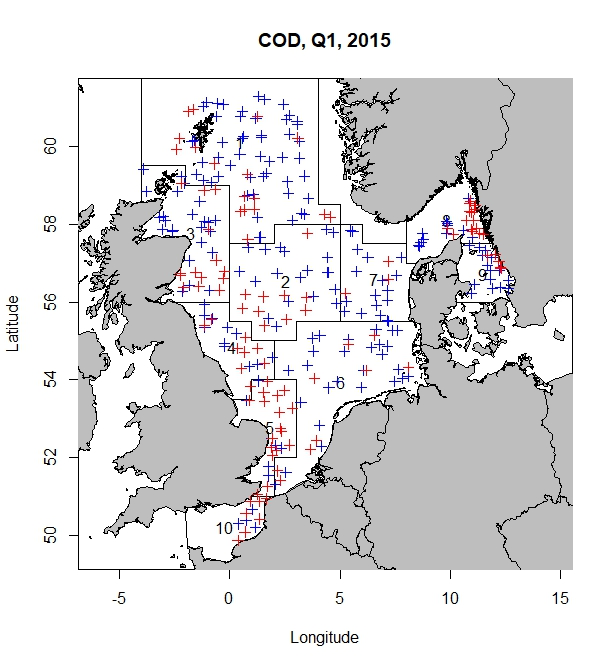
\includegraphics[width=.43\linewidth]{codQ12015Hauls.jpeg}}
    \hfill
\subfloat{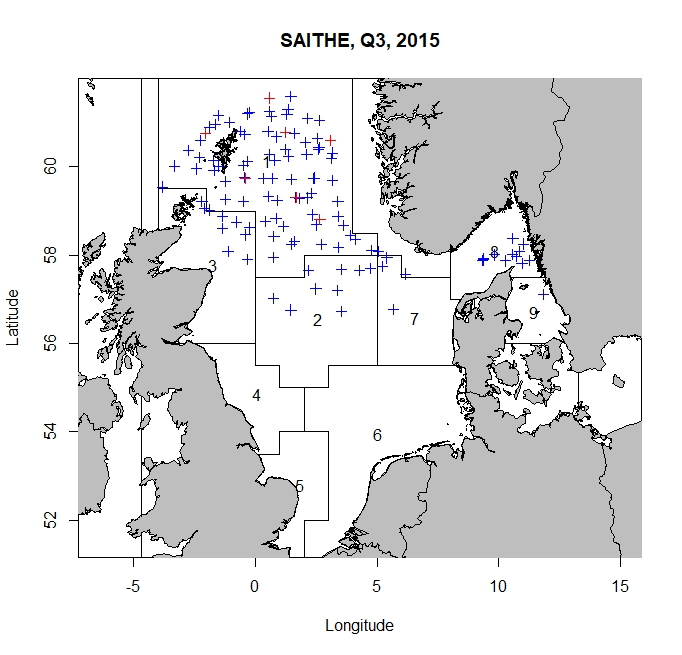
\includegraphics[width=.48\linewidth]{saitheQ32015Hauls.jpeg}}

\subfloat{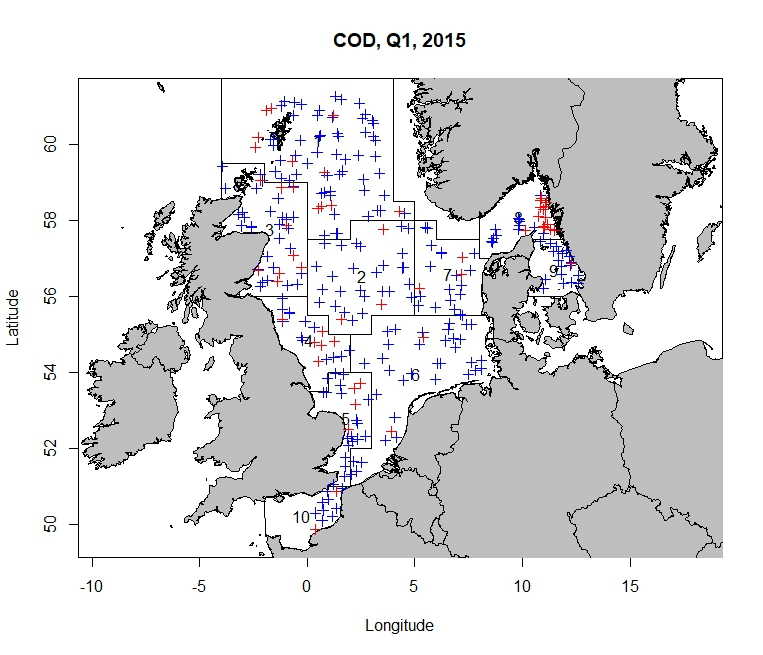
\includegraphics[width=.48\linewidth]{codQ12015Hauls5cm.jpeg}}
    \hfill
\subfloat{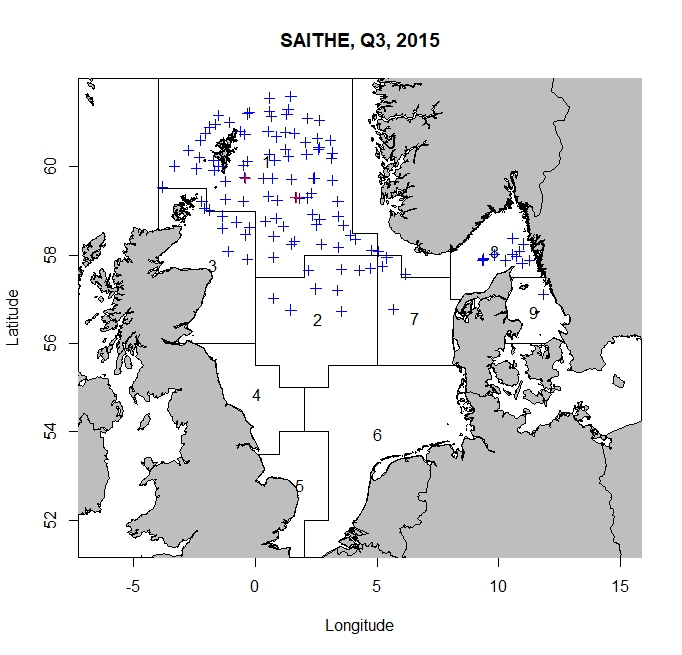
\includegraphics[width=.44\linewidth]{saitheQ32015Hauls5cm.jpeg}}\
    \caption{cod with length class 1 cm (upper left) and length class 5 cm (lower left), and saithe with length class 1cm (upper right) and length class 5 cm (lower right)}
    \label{fig:trawlhauls}
\end{figure}



%the following bootstrap procedures: a bootstrap procedure for sampling lengths as given in the naive procedure 


%\clearpage

%We propose a stratified bootstrap approach, which is similar to the DATRAS bootstrap approach but which preserves  both the number of trawl hauls within each statistical rectangle and the age observations within each length class. The stratified bootstrap procedure is as follows:
%\begin{enumerate}
%\item Assume there are $N_{\text{RFA}}^{(i)}$ trawl hauls in the $i$th statistical rectangle.  Sample with replacement $N_{\text{RFA}}^{(i)}$ of the trawl hauls in the $i$th statistical rectangle. If there is only one trawl haul in the statistical rectangle, sample either that trawl haul or the closest in air distance. 
%\item Repeat step 1 for each statistical rectangle with trawl hauls. 
%\item Sample the catch-at-age (CA)-data with the same procedure as used in the DATRAS procedure.   
%\item Calculate CPUEs 
%\item Repetat step 1-4 B times. 
%\end{enumerate}  
%Both the DATRAS and stratified bootstrap approaches sample age information in the whole RFA. However, given that the ALK is trawl dependent,that is, has a spatial structure on finer scale than the RFA, these procedures will underestimate the uncertainty. 
%
% 
%\subsubsection{Haul-based bootstrap procedure} 
%
%\begin{enumerate}
%\item Assume there are $N_{\text{RFA}}^{(i)}$ trawl hauls in the $i$th statistical rectangle.  Sample with replacement $N_{\text{RFA}}^{(i)}$ of the trawl hauls in the $i$th statistical rectangle, and define ${\bf T}_{\text{sim}}^{\text{length}}$ to be that sample. If there is only one trawl haul in the statistical rectangle, sample either that trawl haul or the closest in air distance. 
%\item If there are no missing age-length compositions in the trawl hauls in the $i$th statistical rectangle calculate CPUEs. 
%\item If there are missing ages in the trawl hauls, then use the imputation procedure in Section \ref{secAp:oursBorrow} in appendix  \ref{sec:imputationappendix}, and then calculate CPUEs.
%\item Repeat steps 1-3 B times for the each statistical rectangle in the RFA 
%\end{enumerate}
%
% 
%\subsubsection{Model-based ALK bootstrap procedure}
%The bootstrap procedure used for calculating confidence intervals for the CPUE with use of the model-based ALK is constructed by sampling hauls stratified with respect to each statistical rectangle. The uncertainty in the ALK is taken into account by sampling from the joint normal approximation of the likelihood in each iteration in the bootstrap procedure. The joint precision matrix needed for the normal approximation is extracted from the estimated model in TMB. 


%{\bf Ratio estimator} 
%
%The aim of this method is to obtain increased precision by taking advantage of the correlation between $x$ and $y$, where $x$ is an auxiliary variate correlated with $y$, that is, $x$ is often the value of $y$ at some previous time when a complete census was taken.
%
%\begin{itemize}
%
%
%\item Clustered samples are not as statistically efficient as simple random samples. 
%
%\item Similarities among subjects in clusters can reduce the variability of responses from a cluster compared with those expected from a simple random sample. 
%
%\item If statistics meant for simple random samples are used to design and analyze clustered studies, they will result in overestimation of the effective sample size.
%
%
%\item most statistical methodologies were designed to analyse data that is both selected and analyse on the same level.
%
%\item Clustered designs can be used for many reasons, but they always cause some loss of statistical efficiency as a result of the “relatedness” within the preexisting groups. 
%
%\item Clustered data result when some preexisting group structure is used to select study participants, but the researcher is interested in the individual level data.
%
%\item the design of fisheries research studies creates clusters. For example, the trawl hauls are "randomized (semi-random)" but the data to be analysed is at the fish level
%
%\item fish caught together are often more similar than those in the general population 
%\item Even low levels of intracluster correlation can greatly increase the variance of an estimate compared with that from a simple random sample 
%\item density of marine mammals is usually highly variable over a region, which in the presence of intracluster correlation contributes significantly to the variance of population parameter estimates
%
%\item to take into account the areal stratification of trawl hauls, a combined ratio estimator  would be appropriate or .... this type of estimator is necessary because the proportion of fish in each stratum is unknown
%\end{itemize}
%

%{\bf Hierarchical versus stratified }
%
%\begin{itemize}
%
%\item Hierarchical data, such as environmetric data, often include multiple sources of variation that can be described using a hierarchical or multilevel model 
%\item  It may be important when setting up a resampling scheme to take careful account of the multiple sources of variation depending on the nature of the parameter being estimated. 
%
%\item For hierarchical unbalanced data having more than two levels, there are more than two bootstrap resampling strategies
%
%\item  The resampling strategy that works best for three-level (or multilevel) data, such as the structure with regions, families, members [7,9] has not yet been determined
%
%\item  Because nonparametric bootstrapping for hierarchical data is not straightforward: certainly it does not make sense to use simple nonparametric resampling, which treats all observations as independent.
%
%\item {(\bf Olav)} As I guessed, the lower and upper bounds of the prediction intervals for the hierarchical procedure is very much larger. If I am right, this is because we typically sample much fewer trawl hauls with the hierarchical procedure than what is taken in reality.
%
%
%\item {(\bf Olav)} Stratified is as follows: The trawl hauls is sampled stratified with respect to statistical rectangles. The ALK is however not calculated with that sample, but by sample the CA-data stratified with respect to age. I think this procedure for sampling ALK was suggested by DATRAS.
% 
%\item {(\bf Olav)} The StratifiedNewALK procedure was something we tried to implement for better accounting for that there may be spatial variation and haul to haul variations in the ALK. It samples trawl hauls stratified with respect to statistical rectangles, and calculate the ALK based on that sample.
% 
%\item {(\bf Olav)} Note that the calculation takes very much time now when procedure = "haulBased", this is because there are many missing ages. We must look more on how to reduce the time needed for that computation. One possible solution could be to use the DATRAS ALK, but substitute the rows were we have observations in the trawl haul. Or borrow strength from trawl hauls in the same statistical rectangle, and if there are no age observations of that length in the statistical rectangle we use the DATRAS ALK for that row.
%
%\item Here is for cod in Q1 in year 2015. By some reason the program failed for Q3 for cod and I don’t see the reason right now and I have to prepare for the AFWG next week.
%
%\item The program does not yet handle fish of age 0, in that sense that the zero year old fish do not contribute to the likelihood. 
%
%\item Here is for saithe. The name of the figures explain which quarter and year. Notice that the 50 cm saithe in Q1 is typically older than the 50cm saithe in Q3, this is reasonable. However, the very little probability of a fish to be of year 2 in Q1 I have to think more on, I have not shown the uncertainty intervals, and there were quite few observations of two year old saithe in Q1.
%
%\item Perhaps we can expand the model to use both quarters at the same time, currently the model is ran separately for each quarter.
%
%\item Note also that it is mostly RFA 1 which is of interest for saithe, that is where most of the saithe is located. 
%
%\item I will send the same figures for cod soon.
%
%\item I have now added code for saithe. I have also removed the pooling (it was luckily just to change that one variable).  However, the program seems to use very much time when using the haul based ALK when we do not pool. This was a bit surprising to me, and it seems to be because there are many missing ages in all the hauls, and R uses time to find the closest trawl hauls. I note this as an “issues” on github. 
% 
%\item I also found an error which seems to remove the error regarding the hierarchical procedure.
% 
%\item The estimates for saithe seems to coincide quite well with datras, but differs slightly. I see that the datras estimates are sometimes positive for Ssaithe even thou there are no observation of that that age in the RFA, this must be something strange (error perhaps, if I have not overseen anything) with the datras estimate. See e.g. RFA 7 in year 2015 in quarter 1. Then it is only observed fish with ages 3,4 and 5, but the estimated CPUE from datras is positive for age equal 2. 
%
%\item So be clear:
%\item currently we are borrowing strength from trawl hauls in the same rectangle or closest rectangle (throughout the RFA) to fill missing ages in the haul-based approach, and if there is no in the whole RFA we used DATRAS extrapolation approach to fill missing data. “
%
%\item Yes. But there is a very small issue I forgot to raise. If there are no observations of the length group in the whole RFA, the ALK from datras is used for that length.  If we extrapolate the haul based ALK for every haul I am a bit afraid that it strange things can happen if there are few age observation in the haul. We can change this so that we extrapolate the ALK for every haul, but then there are some errors I need to handle which I didn’t manage before I went home for the day yesterday. 
%
%\item “Your suggestion is therefore that we borrow strength from trawl hauls within the statistical rectangle, and if there is none we then use DTARAS extrapolation approach to fill missing data? That sounds better to me, because  as we search the entire RFA to fill the missing data it seems to be quite similar to DATRAS with the assumption that age-length structures in the whole RFA are the same.”
%
%\item My suggestion was to use the exact same ALK as used in datras in those cases. If we extrapolate the ALK in a haul with few observation of age (say we only observed a fish of age 1 and 15 cm long in a trawl haul, then fish of size 90 cm in the same trawl haul would also be treated as 1 year old with the haul based extrapolation strategy). 
%
%\item “Also the second sentence in this “Stratified is as follows: The trawl hauls is sampled stratified with respect to statistical rectangles. The ALK is however not calculated with that sample, but by sample the CA-data stratified with respect to age. I think this procedure for sampling ALK was suggested by DATRAS.” Is not clear to me. Do you mean the ALK is computed using DATRAS ALK procedure?” 
%The ALK is calculated with the datras procedure if procedure != "haulBased" and procedure != "hierarchical".  Here I mean that the data that is used for calculating the ALK is sampled stratified with respect to age.
%
%
%
%\end{itemize}
%\clearpage

%As discussed in Section \ref{overview} %We examine the fraction of trawl hauls with length information that had missing age information in Q1 of 2015. 



\clearpage
%\begin{figure}[h!]
%\subfloat[fig 1]{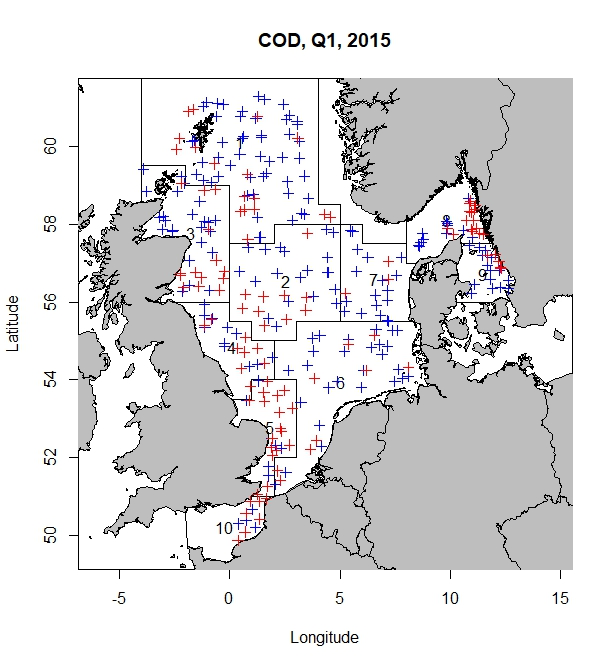
\includegraphics[width = 3in]{codQ12015Hauls.jpeg}} 
%\subfloat[fig 2]{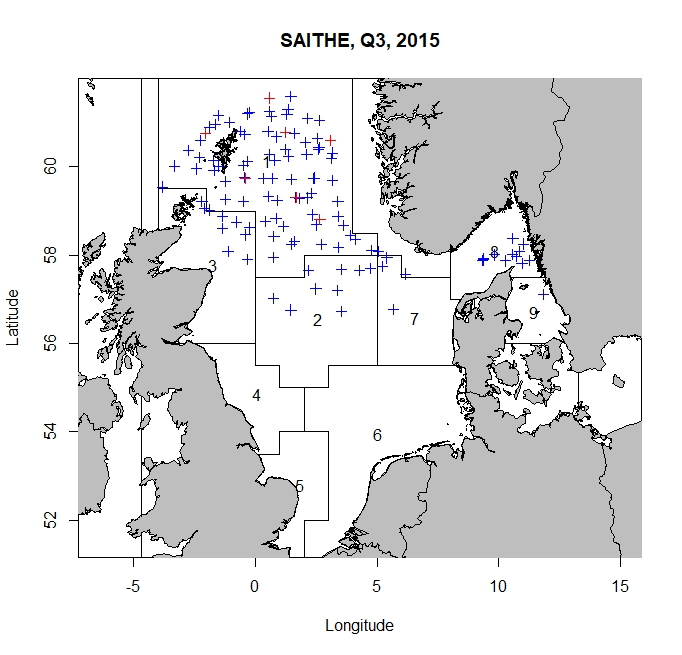
\includegraphics[width = 3in]{saitheQ32015Hauls.jpeg}}\\
%\subfloat[fig 3]{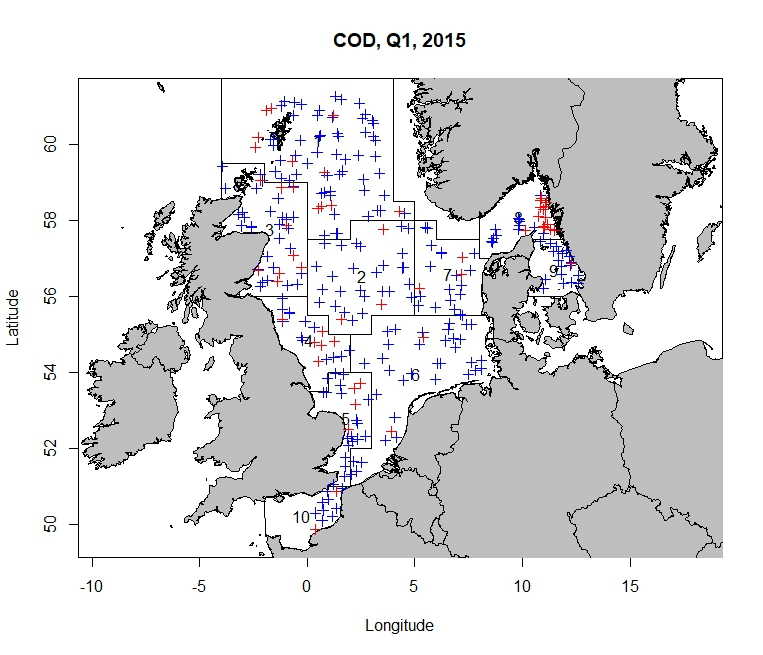
\includegraphics[width = 3in]{codQ12015Hauls5cm.jpeg}}
%\subfloat[fig 4]{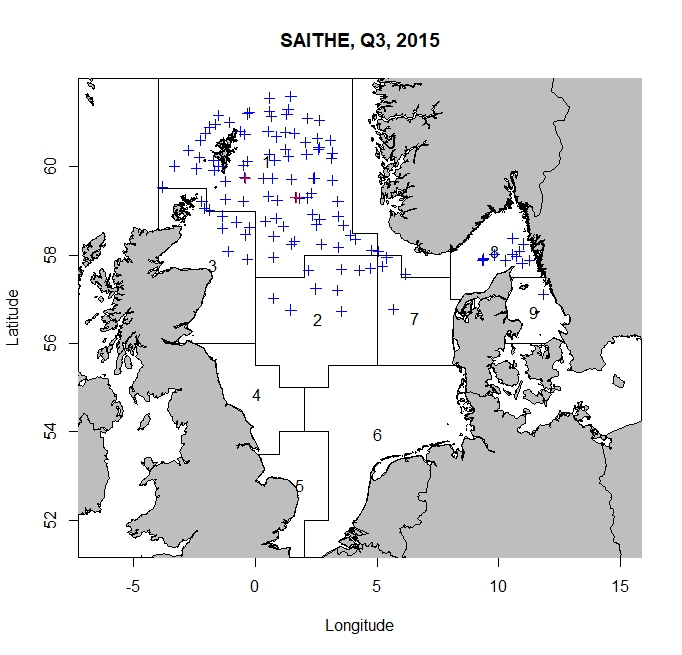
\includegraphics[width = 3in]{saitheQ32015Hauls5cm.jpeg}} 
%\caption{Add your own figures before compiling}
%\label{some example}
%\end{figure}
%%
%
%\begin{figure}
%\centering
%\begin{tabular}{cccc}
%\subfloat{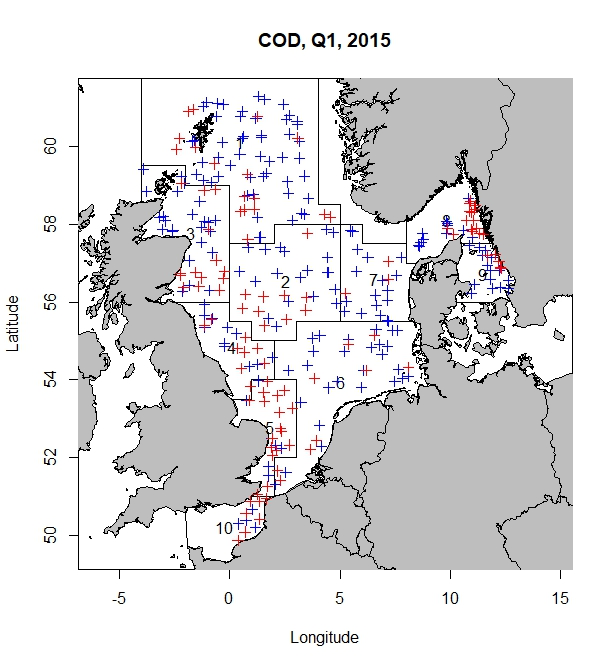
\includegraphics[width=.5\linewidth]{codQ12015Hauls.jpeg}} & 
%\subfloat{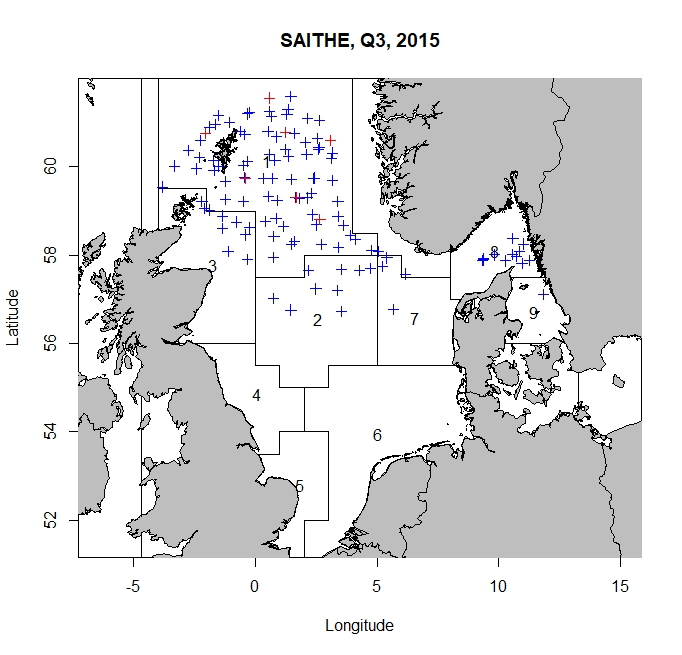
\includegraphics[width=.5\linewidth]{saitheQ32015Hauls.jpeg}} & \\
%\subfloat{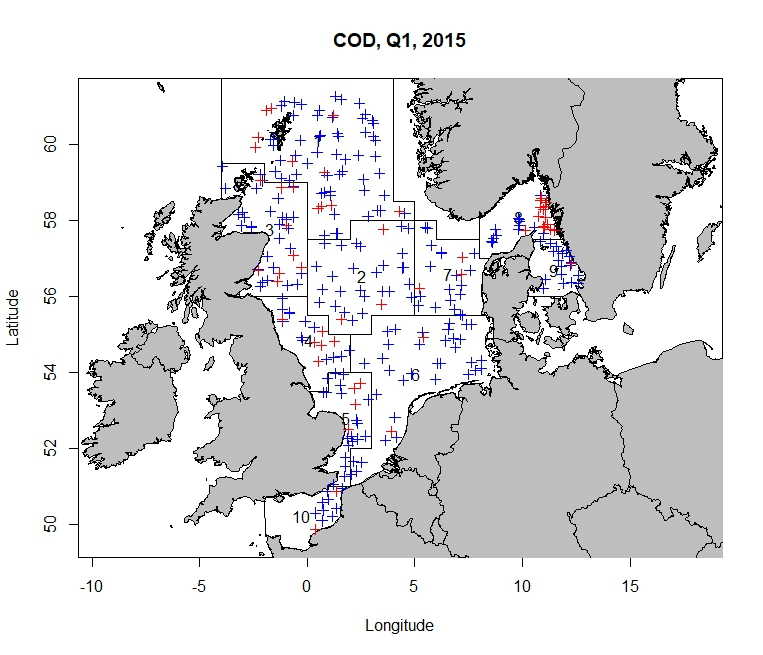
\includegraphics[width=.5\linewidth]{codQ12015Hauls5cm.jpeg}} & 
%\subfloat{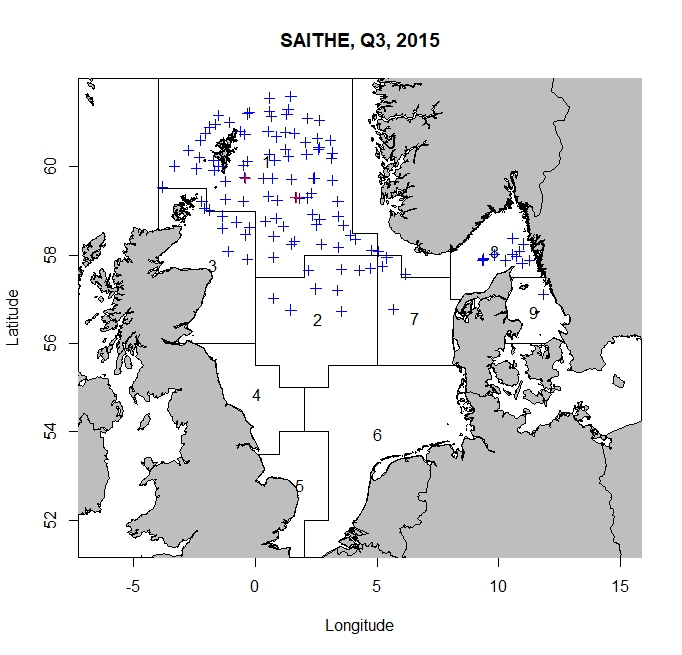
\includegraphics[width=.5\linewidth]{saitheQ32015Hauls5cm.jpeg}}\\
%\end{tabular}
%\caption{correlation}
%\end{figure}



 %for an average of ..days annually. Each nation applies for a given number of ships days funded by Data Collection Framework (DCF), except for Norway who determine their number of survey days \\

%, and on average in quarter 1 ....trawl hauls are taken while ....in quarter 3 are taken. The surveys typically ran for a period of...days \\


%\begin{small}
%\begin{table}[h!]
%\centering
%\captionsetup{font=small, width = 15.5cm}{
%\caption{Survey countries, vessel name, and period research vessels participating in first quarter (Q1) and third quarter (Q3) during 1997-2017.}\label{dayscountries}}
%\begin{tabular}{cccccccc}
%\hline \\[0.1ex]
%  & \multicolumn{2}{c}{\bf average number of sampling days} & \multicolumn{2}{c}{\bf Average number of trawl hauls }\\[1.5ex]
%{\bf Country }  & Q1 & Q3  & Q1 & Q3  \\[0.5ex]
%\cmidrule(lr{0.5em}){1-1}  \cmidrule(lr{0.5em}){2-3}  \cmidrule(lr{0.1em}){4-5} \\ [1ex]
%Denmark     &     &  &    &     \\[1ex]
%France      &     &  &    &    \\[1ex]
%Germany     &     &  &    &    \\[1ex]
%Netherlands &     &  &    &      \\[1ex]
%Norway      & 28  & 21 &   &    \\[1ex]
%Sweden      & 15  &    &   &    \\[1ex]
%UK England  &     &  &    &   \\[1ex]
%UK Scotland &     &  &    &   \\[0.5ex]
%
%\hline
%\end{tabular}
%\end{table}
%\end{small}


\clearpage

\section{RESULTS}
\label{sec:results}

\subsection{Estimates of abundance-at-age and their uncertainty}
\label{sec:resultsabundance}
%The model-based ALK estimator gives the best overall estimation of uncertainty of estimated CPUE as it accounts for spatial differences in age-length structure. As expected the DATRAS estimator gives smaller estimates of the uncertainty in all ages, except ages 3 and 4. The DATRAS ALK estimator lacks the potential to account for spatial differences in the age-length structure, which may be as a consequence of differential growth rates or size-specific migration. The haul-based ALK estimator gives comparable estimates with the the model-based ALK estimator but uncertainty estimates are generally smaller. For all four bootstrap approaches estimated CPUE for all ages is captured within a $95\%$ confidence interval. Note that the nonparametric bootstrap method is advantageous  because it does not assume any distribution for the data, and it also accounts for some of the variability in the sampling distribution of the CPUE, however, there are some limitations of this method. The most important limitation is the assumption that the distribution of the data represented by the sample is a reasonable estimate of the population function from which the data are sampled. If this assumption is violated the random sampling  performed in the bootstrap procedure may add another level of sampling error, resulting in invalid statistical estimations \citep{haukoos2005advanced}. As discussed in Section \ref{overview} the selection of the trawling locations in IBTS is semi-random where cruise leaders selects "clear" tow locations or "blind" tow locations if no clear tow exists by checking the proposed trawl track for hazardous seabed obstructions with acoustic methods. More recently selection of tow locations is based on pre-proposed valid tow locations with start and end positions executed in the period 2000-2017. Hence, the lack of a fully randomized sampling process has the potential to result in biased estimates of parameters and their uncertainty. Random sampling performed in the bootstrap procedure also adds another level of potential sampling error, which is reflected in variation and biased estimates commonly performed in the bootstrap analysis. Note that the sampling distribution of the bootstrapped statistics is frequently not symmetric and computing point estimates from in this manner may reflect biased estimation from the samples. This can be seen in the estimated bootstrap mean values in Table \ref{resultstable}. The percentile method adopted for computing confidence intervals implicitly assumes the sampling distribution of the bootstrapped statistic is symmetric, and a violation of this assumption would caused the coverage to be substantial %(\emph{possibly include median estimates of CPUE to check for skewness or symmetry, and make reference to it. The percentile method also does partial skewness correction, which adds random variability. Possibly check for significant difference between estimates from different estimators? Approximate confidence intervals - as exact nonparametric confidence intervals do not exist for most parameters \citep{bahadur1956nonexistence}}). 


%%\clearpage
%\begin{small}
%\begin{table}[h!]
%\centering
%\scriptsize
%\setlength\tabcolsep{3.5pt} 
%\captionsetup{font=small, width = 15cm}{
%\caption{Estimates of abundance indices (standard error in parentheses) for cod in RFA 1 in the first quarter of year 2015. approximate $95 \%$ confidence intervals (CI) for DATRAS, Naive, Stratified, and Hierarchical bootstrap procedures are also given.}\label{resultstablecod}}
%\begin{tabular}{cccccccccccccccccc}
%\hline \\[0.1ex]
%  & \multicolumn{2}{c}{\bf DATRAS ALK} & \multicolumn{2}{c}{\thead{\bf Haul-Based ALK }} & \multicolumn{2}{c}{\thead{\bf  Model-Based ALK}} \\[1.5ex]
%{\bf Age ($a$) }  & DATRAS &  Naive & Stratified &  Hierarchical & Stratified &  Hierarchical & \\[0.5ex]
%\cmidrule(lr{0.5em}){1-1}  \cmidrule(lr{0.5em}){2-3}  \cmidrule(lr{0.1em}){4-5} \cmidrule(lr{0.5em}){6-7}  \\ [0.1ex]
%1  & 0 (0)         & 0      ( )  &   0 (0)       & 0      ( ) & 0 (0)    &  0 ( )        \\[1ex]
%2  & 0.764  (0.25) & 0.718  ( )  & 0.764  (0.23) & 0.828  ( ) & 0.590 (0.16)  & 0.631  ( )   \\[1ex]
%3  & 21.989 (6.78) & 22.399 ( )  & 21.989 (4.34) & 22.576 ( ) & 22.233 (4.23) & 22.553 ( )  \\[1ex]
%4  & 11.285 (2.20) & 10.385 ( ) & 11.285 (1.27) & 11.878  ( ) & 10.580 (1.23) & 11.532 ( ) \\[1ex]
%5  & 3.265  (0.69) & 2.665  ( ) & 3.265  (0.60) & 3.444   ( ) & 3.656 (0.54)  & 3.740 ( ) \\[1ex]
%6  & 1.147  (0.34) & 0.959  ( ) & 1.147  (0.35) & 1.263   ( ) & 1.267 (0.42)  & 1.448 ( ) \\[1ex]
%7  & 1.276  (0.38) & 0.999  ( ) & 1.276  (0.40) & 1.472   ( )& 1.400 (0.52)  & 1.701  ( ) \\[4.5ex]
%
%
% &&& \multicolumn{3}{c}{\bf Approximate $95 \%$ CI from bootstrap procedures} \\[1.5ex]
%1  & (0, 0)           & (0, 0)           &   (0, 0)          & (0, 0)    & (0, 0)           & (0, 0)          & \\[1ex]
%2  & (0.301, 1.293)   & (0.301, 1.293)   &  (0.405, 1.307)   & (0.405, 1.307)   & (0.324, 0.933)   & (0.354, 1.845)  & \\[1ex]
%3  & (12.673, 38.274) & (12.673, 38.274) & (14.956, 30.131)  & (14.956, 30.131)  & (14.867, 30.043) & (14.531, 30.396)&  \\[1ex]
%4  & (6.661, 15.106)  & (6.661, 15.106)  & (9.613, 14.470)   & (9.613, 14.470)  & (9.215, 13.897)  & (8.383, 15.741) & \\[1ex]
%5  & (1.553, 4.339)   & (1.553, 4.339)   &  (2.329, 4.617)   & (2.329, 4.617)   & (2.797, 4.659)   & (2.025, 5.797)  & \\[1ex]
%6  & (0.424, 1.810)   & (0.424, 1.810)   & (0.637, 1.959)    & (0.637, 1.959)  & (0.644, 2.222)   & (0.540, 2.487)  & \\[1ex]
%7  & (0.387, 1.839)   & (0.387, 1.839)   &  (0.735, 2.299)   &  (0.735, 2.299) & (0.756, 2.644)   & (0.648, 2.286)  & \\[1ex]
%\hline
%\end{tabular}
%\end{table}
%\end{small}
%
%
%\clearpage
%\begin{small}
%\begin{table}[h!]
%\centering
%\scriptsize
%\setlength\tabcolsep{2.8pt} 
%\captionsetup{font=small, width = 16.5cm}{
%\caption{Estimates of abundance indices (standard error in parentheses) for cod in RFA 1 in the first quarter of year 2015. Approximate $95 \%$ confidence intervals (CI) for DATRAS, Naive, Stratified, and Hierarchical bootstrap procedures are also given.}\label{resultstablesaithe}}
%\begin{tabular}{cccccccccccccccccccc}
%\hline \\[0.1ex]
%  & \multicolumn{2}{c}{\bf DATRAS ALK} & \multicolumn{3}{c}{\thead{\bf Haul-based ALK }} & \multicolumn{3}{c}{\thead{\bf  Model-based ALK}} \\[1.5ex]
%{\bf Age ($a$) }  & DATRAS &  Naive & Naive & Stratified &  Hierarchical & Naive &Stratified &  Hierarchical & \\[0.5ex]
%\cmidrule(lr{0.5em}){1-1}  \cmidrule(lr{0.5em}){2-3}  \cmidrule(lr{0.1em}){4-6} \cmidrule(lr{0.5em}){7-9}  \\ [0.1ex]
%1  & 0 (0)         & 0      (0)    & 0       (0)  & 0 (0)        & 0   (0)      & 0 (0)        & 0 (0)        &  0    (0)      \\[1ex]
%2  & 0.764  (0.26) & 0.764  (0.24) & 0.60  (0.23) & 0.60  (0.17) & 0.60  (0.17) & 0.70  (0.34) & 0.70  (0.45) & 0.70  (0.48)   \\[1ex]
%3  & 21.989 (7.30) & 21.989 (3.89) & 22.21 (4.14) & 22.21 (4.19) & 22.21 (4.19) & 22.11 (4.46) & 22.11 (4.10) & 22.11 (13.23)  \\[1ex]
%4  & 11.285 (2.29) & 11.285 (1.30) & 10.58 (1.18) & 10.58 (1.29) & 10.58 (9.60) & 10.99 (2.37) & 10.99 (1.94) & 10.99 (5.20) \\[1ex]
%5  & 3.265  (0.74) & 3.265  (0.57) & 3.67  (1.18) & 3.67  (0.58) & 3.67  (2.00) & 3.50  (0.93) & 3.50  (0.89) & 3.50  (3.28) \\[1ex]
%6  & 1.147  (0.35) & 1.147  (0.37) & 1.27  (0.42) & 1.27  (0.42) & 1.27  (0.91) & 1.20  (0.46) & 1.20  (0.56) & 1.20  (1.28) \\[1ex]
%7  & 1.276  (0.41) & 1.276  (0.40) & 1.40  (0.73) & 1.40  (0.52) & 1.40  (0.85) & 1.21  (0.42) & 1.21  (0.43) & 1.21  (2.63) \\[4.5ex]
%
%
% &&& \multicolumn{4}{c}{\bf Approximate $95 \%$ CI from bootstrap procedures} \\[1.5ex]
%1  &  (0, 0)         & (0, 0)        &(0, 0)        &  (0, 0)          & (0, 0)       & (0, 0) & (0, 0)         & (0, 0)          & \\[1ex]
%2  & (0.27, 1.29)   & (0.40, 1.34)  & (0.31, 1.15)  &  (0.31, 0.93)    & (0, 7.22)    &(0.40, 1.72)  & (0.38, 1.89)   & (0.02, 1.72)  & \\[1ex]
%3  & (12.70, 37.67)  & (15.46, 29.63)& (15.22, 30.25)&  (14.65, 30.18)  & (3.65, 40.02)&(14.33, 3097) & (14.71, 29.90) & (3.71, 54.91)&  \\[1ex]
%4  &  (6.64, 15.33)  & (9.47, 14.32) & (8.94, 13.54) &  (9.14, 13.94)   & (0, 15.63)   &(8.44, 16.60) & (8.65, 16.07)  & (1.84, 21.53) & \\[1ex]
%5  &  (1.56, 4.46)   & (2.43, 4.39)  & (2.46, 6.59)  &  (2.75, 4.77)    & (0, 7.18)    & (2.18, 5.30)  & (1.92, 5.07)  & (0.10, 10.07) \\[1ex]
%6  & (0.39, 1.77)    & (0.64, 1.96)  & (0.39, 2.02)  &  (0.69, 2.27)    & (0, 3.83)    &(0.54, 2.39)  & (0.60, 2.79)   & (0.01, 3.30)  & \\[1ex]
%7  & (0.42, 2.13)    & (0.75, 2.28)  & (0.62, 3.23)  &  (0.78, 2.68)    & (0, 2.38)    &(0.70, 2.30)  & (0.66, 2.26)   & (0., 3.09)  & \\[1ex]
%\hline
%\end{tabular}
%\end{table}
%\end{small}

\begin{tiny}
\begin{table}[h!]
\centering
\scriptsize
\setlength\tabcolsep{1.8pt} 
\captionsetup{font=small, width = 16.5cm}{
\caption{Estimates of abundance indices (Index), and estimated standard errors for 400 bootstrap samples from the following bootstrap procedures: DATRAS, Naive, Stratified, and Hierarchical for cod in RFA 1 in the first quarter of year 2015. Approximate $95 \%$ confidence intervals (CI) are also given.}\label{resultstablesaithe}}
\begin{tabular}{ccccccccccccccccccccccccccc}
\hline \\[0.1ex]
  & \multicolumn{3}{c}{\bf DATRAS ALK} & \multicolumn{3}{c}{\thead{\bf Haul-based ALK }} & \multicolumn{3}{c}{\thead{\bf  Model-based ALK}} \\[1.5ex]
  & \multicolumn{3}{c}{DATRAS Bootstrap}   & \multicolumn{3}{c}{Stratified Bootstrap}   & \multicolumn{3}{c}{Stratified Bootstrap} \\[1.5ex]
   \cmidrule(lr{0.5em}){2-4}  \cmidrule(lr{0.1em}){5-7} \cmidrule(lr{0.5em}){8-10}  \\ [0.1ex]
{\bf Age ($a$) }  &\thead{Abundance \\ estimate} & \thead{Standard \\ error} & \thead{Relative \\ standard error} &\thead{Abundance \\ estimate} & \thead{Standard \\ error} & \thead{Relative \\ standard error} & \thead{Abundance \\ Estimate}  & \thead{Standard \\ error} & \thead{Relative \\ standard error}& \\[0.5ex]
\cmidrule(lr{0.5em}){1-1}  \cmidrule(lr{0.5em}){2-4}  \cmidrule(lr{0.1em}){5-7} \cmidrule(lr{0.5em}){8-10}  \\ [0.1ex]
0  & 0      & 0    & $-$  & 0    &   0   & $-$     & 0    & 0    & $-$         \\[1ex]
1  & 0.764  & 0.26 & $34 \%$ & 0.60  & 0.24 & $40 \%$   & 0.70  & 0.36 & $51 \%$   \\[1ex]
2  & 21.989 & 6.76 & $31 \%$ & 22.21 & 4.15 & $19 \%$   & 22.11 & 4.28 & $19 \%$   \\[1ex]
3  & 11.285 & 2.19 & $19 \%$ & 10.58 & 1.20 & $11 \%$   & 10.99 & 1.77 & $16 \%$ \\[1ex]
4  & 3.265  & 0.71 & $22 \%$ & 3.67  & 1.28 & $35 \%$   & 3.50  & 0.87 & $25 \%$  \\[1ex]
5  & 1.147  & 0.34 & $30 \%$ & 1.27  & 0.42 & $33 \%$   & 1.20  & 0.48 & $40 \%$  \\[1ex]
6+  & 1.276  & 0.38 & $30 \%$ & 1.40  & 0.70 & $50 \%$   & 1.21  & 0.42 & $35 \%$  \\[4.5ex]


 & \multicolumn{8}{c}{\bf Approximate $95 \%$ CI from bootstrap procedures} \\[1.5ex]
0  & 0      &(0, 0)         && 0      &  (0, 0)         && 0     & (0, 0)           \\[1ex]
1  & 0.764  &(0.31, 1.33)   && 0.60   &  (0.31, 0.91)   && 0.70  & (0.35, 1.48)    \\[1ex]
2  & 21.898 &(12.73, 37.15) && 22.21  &  (15.64, 30.72) && 22.11 & (14.76, 30.36) \\[1ex]
3  & 11.285 &(6.31, 15.02)  && 10.58  &  (8.74, 13.65)  && 10.99 & (8.61, 15.42)  \\[1ex]
4  & 3.265  &(1.49, 4.21)   && 3.67   &  (2.81, 4.74)   && 3.50  &(1.96, 5.60)   \\[1ex]
5  & 1.147  &(0.40, 1.75)   && 1.27   &  (0.67, 2.31)   && 1.20  &  (0.56, 2.78)   \\[1ex]
6+  & 1.276  &(0.44, 1.82)   && 1.40   &  (0.78, 2.69)   && 1.21  & (0.70, 2.43)  \\[1ex]
\hline
\end{tabular}
\end{table}
\end{tiny}





\begin{tiny}
\begin{table}[h!]
\centering
\scriptsize
\setlength\tabcolsep{1.8pt} 
\captionsetup{font=small, width = 16.5cm}{
\caption{Estimates of abundance indices (Index), and estimated standard errors for 400 bootstrap samples from the following bootstrap procedures: DATRAS, Naive, Stratified, and Hierarchical for cod in RFA 1 in the first quarter of year 2015. Approximate $95 \%$ confidence intervals (CI) are also given.}\label{resultstablesaithe}}
\begin{tabular}{ccccccccccccccccccccccccccc}
\hline \\[0.1ex]
  & \multicolumn{3}{c}{\bf DATRAS ALK} & \multicolumn{4}{c}{\thead{\bf Haul-based ALK }} & \multicolumn{4}{c}{\thead{\bf  Model-based ALK}} \\[1.5ex]
{\bf Age ($a$) }  &Index & DATRAS &  Naive &Index & Naive & Stratified &  Hierarchical &Index & Naive &Stratified &  Hierarchical & \\[0.5ex]
\cmidrule(lr{0.5em}){1-1}  \cmidrule(lr{0.5em}){2-4}  \cmidrule(lr{0.1em}){5-8} \cmidrule(lr{0.5em}){9-12}  \\ [0.1ex]
1  & 0      & 0    & 0            & 0    &   0  & 0     & 0     & 0           & 0         &  0   & 0       \\[1ex]
2  & 0.764  & 0.26 & 0.23 & 0.60  & 0.24 & 0.16 & 0.81  & 0.70  & 0.36 & 0.31 & 0.78   \\[1ex]
3  & 21.989 & 6.76 & 4.08 & 22.21 & 4.15 & 4.20 & 13.23 & 22.11 & 4.28 & 4.26 & 10.69  \\[1ex]
4  & 11.285 & 2.19 & 1.27 & 10.58 & 1.20 & 1.28 & 5.85  & 10.99 & 1.77 & 1.84 & 4.53 \\[1ex]
5  & 3.265  & 0.71 & 0.57 & 3.67  & 1.28 & 0.56 & 3.02  & 3.50  & 0.87 & 0.94 & 2.46 \\[1ex]
6  & 1.147  & 0.34 & 0.33 & 1.27  & 0.43 & 0.43 & 1.59  & 1.20  & 0.48 & 0.62 & 0.83 \\[1ex]
7  & 1.276  & 0.38 & 0.39 & 1.40  & 0.70 & 0.53 & 2.01  & 1.21  & 0.42 & 0.46 & 0.85 \\[4.5ex]


 &&& \multicolumn{8}{c}{\bf Approximate $95 \%$ CI from bootstrap procedures} \\[1.5ex]
1  & 0      &(0, 0)         & (0, 0)        & 0     &(0, 0)         &  (0, 0)         & (0, 0)        & 0     &(0, 0)        & (0, 0)         & (0, 0)   \\[1ex]
2  & 0.764  &(0.31, 1.33)   & (0.40, 1.22)  & 0.60  &(0.20, 1.18)   &  (0.31, 0.91)   & (0, 3.81)     & 0.70  &(0.37, 1.81)  & (0.35, 1.48)   & (0.05, 2.05) \\[1ex]
3  & 21.898 &(12.73, 37.15) & (14.90, 30.01)& 22.21 &(15.01, 30.09) &  (15.64, 30.72) & (11.34, 61.57)& 22.11 &(14.56, 30.61)& (14.76, 30.36) & (7.12, 41.41)\\[1ex]
4  & 11.285 &(6.31, 15.02)  & (9.63, 14.42) & 10.58 &(8.75, 13.54)  &  (8.74, 13.65)  & (0, 17.73)    & 10.99 &(8.45, 15.43) & (8.61, 15.42)  & (3.90, 19.99)\\[1ex]
5  & 3.265  &(1.49, 4.21)   & (2.45, 4.50)  & 3.67  &(2.42, 7.35)   &  (2.81, 4.74)   & (0, 8.26)     & 3.50  &(2.11, 5.56)  & (1.96, 5.60)   & (0.87, 8.10)\\[1ex]
6  & 1.147  &(0.40, 1.75)   & (0.67, 1.95)  & 1.27  &(0.50, 2.14)   &  (0.67, 2.31)   & (0, 4.35)     & 1.20  & (0.58, 2.50) & (0.56, 2.78)   & (0.15, 2.98)\\[1ex]
7  & 1.276  &(0.44, 1.82)   & (0.72, 2.24)  & 1.40  &(0.71, 3.42)   &  (0.78, 2.69)   & (0, 5.15)     & 1.21  &(0.70, 2.27)  & (0.70, 2.43)   & (0.09, 3.22) \\[1ex]
\hline
\end{tabular}
\end{table}
\end{tiny}

\clearpage

%\clearpage
\begin{small}
\begin{table}[h!]
\centering
\scriptsize
\setlength\tabcolsep{1.8pt} 
\captionsetup{font=small, width = 16.5cm}{
\caption{Estimates of abundance indices (Index), and estimated standard errors for 200 bootstrap samples from the following bootstrap procedures: DATRAS, Naive, Stratified, and Hierarchical for cod in RFA 1 in the first quarter of year 2015. Approximate $95 \%$ confidence intervals (CI) are also given.}\label{resultstablesaithe}}
\begin{tabular}{ccccccccccccccccccccccccccc}
\hline \\[0.1ex]
  & \multicolumn{3}{c}{\bf DATRAS ALK} & \multicolumn{4}{c}{\thead{\bf Haul-based ALK }} & \multicolumn{4}{c}{\thead{\bf  Model-based ALK}} \\[1.5ex]
{\bf Age ($a$) }  &Index & DATRAS &  Naive &Index & Naive & Stratified &  Hierarchical &Index & Naive &Stratified &  Hierarchical & \\[0.5ex]
\cmidrule(lr{0.5em}){1-1}  \cmidrule(lr{0.5em}){2-4}  \cmidrule(lr{0.1em}){5-8} \cmidrule(lr{0.5em}){9-12}  \\ [0.1ex]
1  & 0     & 0         & 0          & 0    &   0  & 0         & 0         & 0         & 0         &  0   & 0       \\[1ex]
2  & 0.764  & 0.26 & 0.24 & 0.60  & 0.23 & 0.17 & 2.55 & 0.70  & 0.34 & 0.45 & 0.48   \\[1ex]
3  & 21.989 & 7.30 & 3.89 & 22.21 & 4.14 & 4.19 & 9.61 & 22.11 & 4.46 & 4.10 & 13.23  \\[1ex]
4  & 11.285 & 2.29 & 1.30 & 10.58 & 1.18 & 1.29 & 4.72 & 10.99 & 2.37 & 1.94 & 5.20 \\[1ex]
5  & 3.265  & 0.74 & 0.57 & 3.67  & 1.18 & 0.58 & 2.00 & 3.50  & 0.93 & 0.89 & 3.28 \\[1ex]
6  & 1.147  & 0.35 & 0.37 & 1.27  & 0.42 & 0.42 & 0.91 & 1.20  & 0.46 & 0.56 & 1.28 \\[1ex]
7  & 1.276  & 0.41 & 0.40 & 1.40  & 0.73 & 0.52 & 0.85 & 1.21  & 0.42 & 0.43 & 2.63 \\[4.5ex]


 &&& \multicolumn{8}{c}{\bf Approximate $95 \%$ CI from bootstrap procedures} \\[1.5ex]
1  & 0      &(0, 0)          & (0, 0)        & 0     &(0, 0)          &  (0, 0)          & (0, 0)       & 0     &(0, 0) & (0, 0)         & (0, 0)          & \\[1ex]
2  & 0.764  & (0.27, 1.29)   & (0.40, 1.34)  & 0.60  &(0.31, 1.15)    &  (0.31, 0.93)    & (0, 7.22)    & 0.70  &(0.40, 1.72)  & (0.38, 1.89)   & (0.02, 1.72) \\[1ex]
3  & 21.898 & (12.70, 37.67) & (15.46, 29.63)& 22.21 & (15.22, 30.25) &  (14.65, 30.18)  & (3.65, 40.02)& 22.11 &(14.33, 3097) & (14.71, 29.90) & (3.71, 54.91)\\[1ex]
4  & 11.285 &(6.64, 15.33)   & (9.47, 14.32) & 10.58 &(8.94, 13.54)   &  (9.14, 13.94)   & (0, 15.63)   & 10.99 &(8.44, 16.60) & (8.65, 16.07)  & (1.84, 21.53)\\[1ex]
5  & 3.265  &(1.56, 4.46)    & (2.43, 4.39)  & 3.67  &(2.46, 6.59)    &  (2.75, 4.77)    & (0, 7.18)    & 3.50  &(2.18, 5.30)  & (1.92, 5.07)   & (0.10, 10.07)\\[1ex]
6  & 1.147  &(0.39, 1.77)    & (0.64, 1.96)  & 1.27  & (0.39, 2.02)   &  (0.69, 2.27)    & (0, 3.83)    & 1.20  & (0.54, 2.39)  & (0.60, 2.79)   & (0.01, 3.30)\\[1ex]
7  & 1.276  &(0.42, 2.13)    & (0.75, 2.28)  & 1.40  &(0.62, 3.23)    &  (0.78, 2.68)    & (0, 2.38)    & 1.21  &(0.70, 2.30)  & (0.66, 2.26)   & (0., 3.09) \\[1ex]
\hline
\end{tabular}
\end{table}
\end{small}



%\clearpage
\begin{small}
\begin{table}[h!]
\centering
\scriptsize
\setlength\tabcolsep{1.8pt} 
\captionsetup{font=small, width = 16.5cm}{
\caption{Estimates of abundance indices (Index), and estimated standard errors from the following bootstrap procedures: DATRAS, Naive, Stratified, and Hierarchical for saithe in RFA 1 in the third quarter of year 2015. Approximate $95 \%$ confidence intervals (CI) are also given.}\label{resultstablesaithe}}
\begin{tabular}{ccccccccccccccccccccccccccc}
\hline \\[0.1ex]
  & \multicolumn{3}{c}{\bf DATRAS ALK} & \multicolumn{4}{c}{\thead{\bf Haul-based ALK }} & \multicolumn{4}{c}{\thead{\bf  Model-based ALK}} \\[1.5ex]
{\bf Age ($a$) }  &Index & DATRAS &  Naive &Index & Naive & Stratified &  Hierarchical &Index & Naive &Stratified &  Hierarchical & \\[0.5ex]
\cmidrule(lr{0.5em}){1-1}  \cmidrule(lr{0.5em}){2-4}  \cmidrule(lr{0.1em}){5-8} \cmidrule(lr{0.5em}){9-12}  \\ [0.1ex]
1  & 0     & 0         & 0          & 0    &   0  & 0         & 0         & 0         & 0         &  0   & 0       \\[1ex]
2  & 0.764  & 0.26 & 0.24 & 0.60  & 0.23 & 0.17 & 2.55 & 0.70  & 0.34 & 0.45 & 0.48   \\[1ex]
3  & 21.989 & 7.30 & 3.89 & 22.21 & 4.14 & 4.19 & 9.61 & 22.11 & 4.46 & 4.10 & 13.23  \\[1ex]
4  & 11.285 & 2.29 & 1.30 & 10.58 & 1.18 & 1.29 & 4.72 & 10.99 & 2.37 & 1.94 & 5.20 \\[1ex]
5  & 3.265  & 0.74 & 0.57 & 3.67  & 1.18 & 0.58 & 2.00 & 3.50  & 0.93 & 0.89 & 3.28 \\[1ex]
6  & 1.147  & 0.35 & 0.37 & 1.27  & 0.42 & 0.42 & 0.91 & 1.20  & 0.46 & 0.56 & 1.28 \\[1ex]
7  & 1.276  & 0.41 & 0.40 & 1.40  & 0.73 & 0.52 & 0.85 & 1.21  & 0.42 & 0.43 & 2.63 \\[4.5ex]


 &&& \multicolumn{8}{c}{\bf Approximate $95 \%$ CI from bootstrap procedures} \\[1.5ex]
1  & 0      &(0, 0)          & (0, 0)        & 0     &(0, 0)          &  (0, 0)          & (0, 0)       & 0     &(0, 0) & (0, 0)         & (0, 0)          & \\[1ex]
2  & 0.764  & (0.27, 1.29)   & (0.40, 1.34)  & 0.60  &(0.31, 1.15)    &  (0.31, 0.93)    & (0, 7.22)    & 0.70  &(0.40, 1.72)  & (0.38, 1.89)   & (0.02, 1.72) \\[1ex]
3  & 21.898 & (12.70, 37.67) & (15.46, 29.63)& 22.21 & (15.22, 30.25) &  (14.65, 30.18)  & (3.65, 40.02)& 22.11 &(14.33, 3097) & (14.71, 29.90) & (3.71, 54.91)\\[1ex]
4  & 11.285 &(6.64, 15.33)   & (9.47, 14.32) & 10.58 &(8.94, 13.54)   &  (9.14, 13.94)   & (0, 15.63)   & 10.99 &(8.44, 16.60) & (8.65, 16.07)  & (1.84, 21.53)\\[1ex]
5  & 3.265  &(1.56, 4.46)    & (2.43, 4.39)  & 3.67  &(2.46, 6.59)    &  (2.75, 4.77)    & (0, 7.18)    & 3.50  &(2.18, 5.30)  & (1.92, 5.07)   & (0.10, 10.07)\\[1ex]
6  & 1.147  &(0.39, 1.77)    & (0.64, 1.96)  & 1.27  & (0.39, 2.02)   &  (0.69, 2.27)    & (0, 3.83)    & 1.20  & (0.54, 2.39)  & (0.60, 2.79)   & (0.01, 3.30)\\[1ex]
7  & 1.276  &(0.42, 2.13)    & (0.75, 2.28)  & 1.40  &(0.62, 3.23)    &  (0.78, 2.68)    & (0, 2.38)    & 1.21  &(0.70, 2.30)  & (0.66, 2.26)   & (0., 3.09) \\[1ex]
\hline
\end{tabular}
\end{table}
\end{small}


\subsection{Optimum Sampling Effort for North Sea cod and saithe}
\label{sec:resultsoptim}

%
%\clearpage
%\begin{small}
%\begin{table}[h!]
%\centering
%\scriptsize
%\setlength\tabcolsep{0.5pt} 
%\captionsetup{font=small, width = 16cm}{
%\caption{Estimates of abundance indices ($\mathrm{mCPUE}_{1,a}$) and the estimated bootstrap mean ($\mathrm{boot.mCPUE}_{1,a}$) for cod in RFA 1 in the first quarter of year 2015. Estimated average standard error estimates of the $\mathrm{mCPUE}_{1,a}$ are given in parentheses, and $95 \%$ confidence intervals (CI) for DATRAS, and Stratified, Haul-based and Model-based bootstrap procedures are also given.}\label{resultstable}}
%\begin{tabular}{cccccccccccccccccc}
%\hline \\[0.1ex]
%  & \multicolumn{2}{c}{\bf DATRAS} & \multicolumn{2}{c}{\thead{\bf Stratified }} & \multicolumn{2}{c}{\thead{\bf  Haul-based}} & \multicolumn{2}{c}{\thead{\bf  Model-based}}\\[1.5ex]
%{\bf Age ($a$) }  & $\mathrm{mCPUE}_{1,a}$ &  $\mathrm{boot.mCPUE}_{1,a}$ & $\mathrm{mCPUE}_{1,a}$ &  $\mathrm{boot.mCPUE}_{1,a}$ & $\mathrm{mCPUE}_{1,a}$ &  $\mathrm{boot.mCPUE}_{1,a}$ &  $\mathrm{mCPUE}_{1,a}$ &  $\mathrm{boot.mCPUE}_{1,a}$\\[0.5ex]
%\cmidrule(lr{0.5em}){1-1}  \cmidrule(lr{0.5em}){2-3}  \cmidrule(lr{0.5em}){4-5} \cmidrule(lr{0.5em}){6-7}  \cmidrule(lr{0.5em}){8-9}\\ [0.1ex]
%1  & 0 (0)     & 0      &   0 (0)       & 0      & 0 (0)    &  0     &  0 (0)  & 0    \\[1ex]
%2  & 0.764  (0.25) & 0.718  & 0.764  (0.23) & 0.828  & 0.590 (0.16)  & 0.631  & 0.704 (0.40) & 0.924 \\[1ex]
%3  & 21.989 (6.78) & 22.399 & 21.989 (4.34) & 22.576 & 22.233 (4.23) & 22.553 & 22.113 (4.21) & 22.242 \\[1ex]
%4  & 11.285 (2.20) & 10.385  & 11.285 (1.27) & 11.878 & 10.580 (1.23) & 11.532 & 10.995 (1.94) & 11.798 \\[1ex]
%5  & 3.265  (0.69) & 2.665  & 3.265  (0.60) & 3.444  & 3.656 (0.54)  & 3.740  & 3.501 (0.97) & 3.642 \\[1ex]
%6  & 1.147  (0.34) & 0.959  & 1.147  (0.35) & 1.263  & 1.267 (0.42)  & 1.448  & 1.199 (0.51)& 1.327\\[1ex]
%7  & 1.276  (0.38) & 0.999  & 1.276  (0.40) & 1.472  & 1.400 (0.52)  & 1.701  & 1.215 (0.43) & 1.379\\[4.5ex]
%
%
% &&& \multicolumn{4}{c}{\bf Approximate $95 \%$ CI from bootstrap procedures} \\[1.5ex]
%1  & (0, 0)           & &   (0, 0)          & & (0, 0)           & &(0, 0)          & \\[1ex]
%2  & (0.301, 1.293)   & &  (0.405, 1.307)   & & (0.324, 0.933)   & &(0.354, 1.845)  & \\[1ex]
%3  & (12.673, 38.274) & & (14.956, 30.131)  & & (14.867, 30.043) & &(14.531, 30.396)&  \\[1ex]
%4  & (6.661, 15.106)  & & (9.613, 14.470)   & & (9.215, 13.897)  & &(8.383, 15.741) & \\[1ex]
%5  & (1.553, 4.339)   & &  (2.329, 4.617)   & & (2.797, 4.659)   & &(2.025, 5.797)  & \\[1ex]
%6  & (0.424, 1.810)   & & (0.637, 1.959)    & & (0.644, 2.222)   & &(0.540, 2.487)  & \\[1ex]
%7  & (0.387, 1.839)   & &  (0.735, 2.299)   & & (0.756, 2.644)   & &(0.648, 2.286)  & \\[1ex]
%\hline
%\end{tabular}
%\end{table}
%\end{small}

%However, the coverage error is
%often substantial if the distribution of ˆθ is not nearly symmetric, however, other meth
%Another limitation of the nonparametric bootstrap method is 
% that the smaller the original sample the less likely it is to represent the entire population,
%thus the more difficult it becomes to compute valid confidence intervals. Note that the
%bootstrap relies heavily on the tails of the estimated sampling distribution when computing
%confidence intervals, and using small samples may jeopardize the validity of this computation.
% The percentile method uses the frequency histogram of the m statistics computed from the bootstrap samples. The 2.5 and 97.5 percentiles constitute the limits of the 95% confidence intervalThe BCa method adjusts for bias in the bootstrapped sampling distributions relative to the actual sampling distribution, and is thus considered a substantial improvement over the percentile method.8 The BCa confidence interval is an adjustment of the percentiles used in the percentile method based upon the calculation of two coefficients called ‘‘bias correction’’ and ‘‘acceleration.’’ The bias correction coefficient adjusts for the skewness in the bootstrap sampling distribution. If the bootstrap sampling distribution is perfectly symmetric, then the bias correction will be zero. The acceleration coefficient adjusts for nonconstant variances within the resampled data sets. As the number of resampled data sets decreases, more variability is introduced into the confidence interval estimation (i.e., the variability is inversely related to the number of resampled data sets).
% It is worth noting that the  only difference between stratified bootstrap approach and the DATRAS appraoch is the sampling of hauls 

% for the sampling variability in the age-length compositions 
%Estimates of CPUE are similar for the three ALK estimators
%%The percentile method implicitly assumes the sampling distribution of T = t(x) is symmetric, but not necessarily normal, and centred at θ = t(P) (unbiased). However, the coverage error is
%%often substantial if the distribution of ˆθ is not nearly symmetric.
%Estimates of abundance indices are computed using 1000 bootstrap replicates.
%
%
%\emph{possibly include median estimates of CPUE to check for skewness or symmetry}



\clearpage

\section{DISCUSSION}
\label{sec:discussion}
\begin{itemize}
\item We have investigated three ALK estimators: 1) DATRAS ALK, 2)Haul-based ALK and 3) Model-based ALK
\item discuss ALK estimators, which of the three is the most appropriate at this time, discuss  model-based ALK and compare with \citet{berg2012spatial} as they are similar are both used on IBTS data
\item How can estimators be improved, also computational time (1000 bootstrapped samples for each of the four estimators took hours (possibly more than ten, needs verification))
\item Possibly consider hierarchical bootstrapping as done in \citet{ren2010nonparametric} - draft codes are available
\item Discuss next steps for example, removal of otoliths or age information and trawl hauls: the effect may be substantial for larger fish (hence older fish) - as shown in table \ref{agelengthcomposition} fewer older fish are sampled and many younger ones are sampled so the effect would be marginal for younger fish). Draft codes are available for this. \citet{wieland2009estimating} found that considerable catches for cod of older ages were made where the IBTS reported low densities or no cod all (\emph{this is based on data from collaborative fishermen-biologists project on cod in the north-eastern central North Sea}). Also smaller sample sizes would also have an effect on estimated bootstrapped confidence intervals. The smaller the original sample the less likely it is to represent the entire population, thus the more difficult it becomes to compute valid confidence intervals. The bootstrap relies heavily on the tails of the estimated sampling distribution when computing confidence intervals, and using small samples may jeopardize the validity of this computation.  
\item a possible full model-based approach for estimating abundance at age with variance simultaneously?
\item \emph{Note to us: include ICES references}
\end{itemize}



\clearpage

\bibliographystyle{apalike}
\bibliography{ibtsBib}

\clearpage

\begin{appendices}

\section{\large Probability Plot for saithe in the North Sea in Q1 of 2015}
\label{secAp:saithe2015Q1Map}

\begin{figure}[h!]
  \centering
 {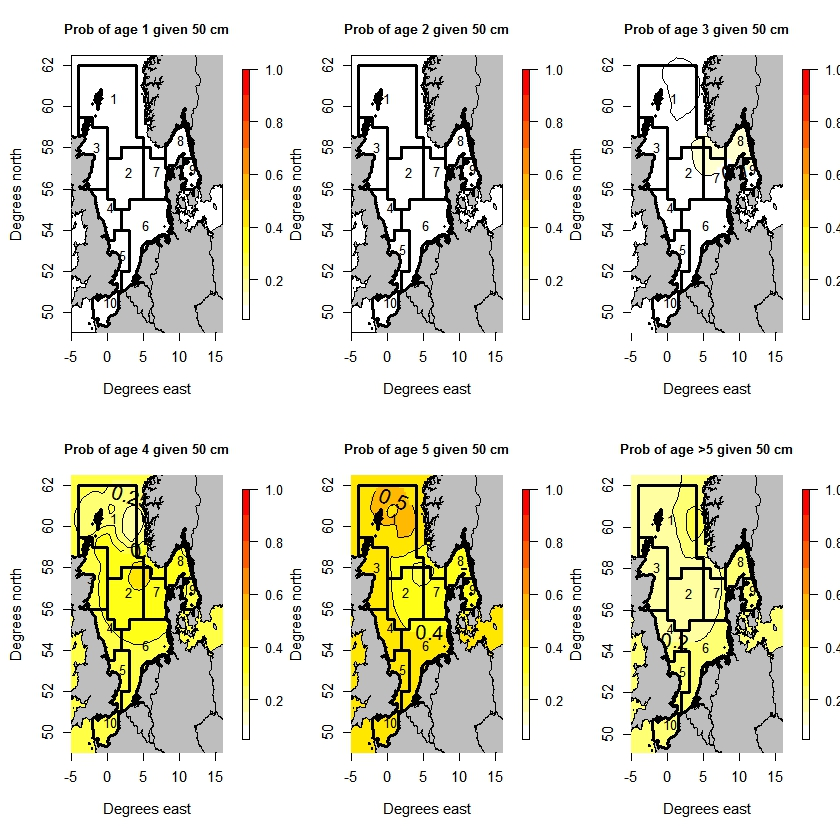
\includegraphics[width=15.5cm]{saithe2015Q1Map.jpeg}}   
 \captionsetup{font= footnotesize, width=15cm}{
 \caption{Estimated probability of age of a 50 cm long saithe in the first quarter of year 2015. The probability of age 1 to age 3 is approximately zero. The polygones marked 1 to 10 is the round fish areas (RFAs) where the ALK is assumed constant in the currently used estimators of the official CPUEs. The plots show that the age of saithe is more likely to be 5 given that it is 50 cm, particularly in RFA 1.}\label{saithe2015Q1Map}}
\end{figure}

\clearpage
%\appendix
\section{\large Areas fished by different countries in the North Sea IBTS}
\label{areasfishedappendix}
Typically, two different countries fish each rectangle so that at least two trawl hauls are made per rectangle. But, intensified sampling is carried out in the following areas: at least 3 hauls per rectangle are taken in statistical rectangles  31F1, 31F2, 32F1, 33F4, 34F2, 34F3, 34F4, 35F3, 35F4; while six or more hauls per rectangle are taken in statistical rectangles  30F1, 32F2, 32F3, 33F2, 33F3 (ICES 1999).  The Skagerrak and Kattegat is fished solely by Sweden, who sample more than once in every rectangle while the west of Shetland (in Q1 and Q3) and inshore areas (Q3) is fished solely by Scotland. The edge of the Norwegian Trench is fished solely by Norway, but inshore areas near Denmark is fished by Denmark. The southern North Sea is fished by Denmark, Germany and England. France, typically, is the only country that surveys the western English Channel. Areas are surveyed by a single country because of the large proportion of untrawalable area (and subsequent gear damage issues experienced by other nations)  for efficient logistical purposes. Table \ref{countries} gives the countries and research vessels participating the North Sea IBTS.\\
\begin{small}
\begin{table}[h!]
\centering
\captionsetup{font=small, width = 15.5cm}{
\caption{Survey countries, vessel name, and period research vessels participating in first quarter (Q1) and third quarter (Q3) during 1997-2017.}\label{countries}}
\begin{tabular}{cccccccc}
\hline \\[0.1ex]
  & \multicolumn{2}{c}{\bf First Quarter (Q1)} & \multicolumn{2}{c}{\bf Third Quarter (Q3)}\\[1.5ex]
{\bf Country }  & Vessel name & Period    & Vessel name & Period  \\[0.5ex]
\hline \\[0.5ex]
Denmark  &   Dana   &   January-February  & Dana & July-August    \\[1ex]
France  & Thalassa II & January-February & - & -   \\[1ex]
Germany   &  Walther  Herwig III & January-February   &   Walther  Herwig III & July-August \\[1ex]
Netherlands &  Tridens 2 &  January-February   & - & -     \\[1ex]
Norway  &   G.O. Sars  & January-February &    Johan Hjort  & July   \\[1ex]
UK England &- & -&  Endeavour &  August-September  \\[1ex]
UK Scotland   &  Scotia III &  January-February & Scotia III &  July-August \\[1ex]
Sweden  &  Dana &  January-February  &  Dana &  August                  \\[0.5ex]
\hline
\end{tabular}
\end{table}
\end{small}

\section{\large Otolith sampling per fish species}
\label{secAp:otolithappendix}
From 1991-2017, most countries conducted quota sampling of otoliths per length group in a RFA. But from 2013 Norway has been sampling one otolith per length class from each trawl haul (to 0.1$\cm$ below for shellfish, to 0.5$\cm$ below for herring and sprat and to 1$\cm$ below for all other species). From the first quarter in 2018 all countries are required to sample one otolith per length class per trawl haul.  Table \ref{otolithsTable} gives the minimum sampling levels of otoliths for the target species. However, for the smallest size groups, that presumably contain only one age group, the number of otoliths per length class may be reduced, and more otoliths per length are required for the larger length classes. \\
\begin{small}
\begin{table}[h!]
\centering
\caption{Minimum sampling levels of otoliths by species for RFA or per trawl haul.}
\label{otolithsTable}
\begin{tabularx}{\linewidth}{r l l l l X}
\toprule 
Period &  Species  & Minimum sampling levels of otoliths per length class    \\[0.7ex]
\midrule \\[0.1ex]
{\bf 1991-2017} & & {\bf Number of otoliths per length class in a RFA}  \\[1.8ex]
     & herring  &  $8$  otoliths per $\frac{1}{2}$ cm group \\[0.8ex]
     & sprat    & $16$  otoliths per $\frac{1}{2}$ cm length class  $8.0 -11.0$ cm\\[0.8ex]
              & & $12$  otoliths per $\frac{1}{2}$ cm length class  $\geq 11.0$ cm\\[0.8ex]
& mackerel      & $8$  otoliths per $\frac{1}{2}$ cm length class \\[0.8ex]
& cod       	  & $8$  otoliths per $1$ cm length class\\[0.8ex]
&haddock   	  & $8$  otoliths per $1$ cm length class \\[0.8ex]
&whiting    	  & $8$  otoliths per $1$ cm length class \\[0.8ex]
&Norway pout   & $8$  otoliths per $1$ cm length class\\[0.8ex]
&saithe        & $8$  otoliths per $1$ cm length class \\[2ex] 
& All target species      &  From 2013 Norway and Scotland, and  Netherlands from 2016 \\[0.7ex] 
&& have been sampling 1 otoliths per length class from each trawl haul \\[0.7ex] 
&& (to 0.1$\cm$ below for shellfish, to 0.5$\cm$ below for herring and sprat, and \\ [0.7ex] 
&& to 1$\cm$ below for all other species).\\[2.7ex] 

{\bf 2018} & & {\bf Number of otoliths per length class per trawl haul}  \\[1.8ex]
  & herring  &  $1$  otoliths per $\frac{1}{2}$ cm group \\[0.8ex]
     & sprat    & $1$  otoliths per $\frac{1}{2}$ cm length class  $8.0 -11.0$ cm\\[0.8ex]
              & & $1$  otoliths per $\frac{1}{2}$ cm length class  $\geq 11.0$ cm\\[0.8ex]
& mackerel      & $1$  otoliths per $1$ cm length class \\[0.8ex]
& cod       	  & $1$  otoliths per $1$ cm length class\\[0.8ex]
& haddock & $2$  otoliths per $5$ cm length class $11 -15, \ 16-20, \ 21-25, \ 26-30$ cm \\[0.8ex]
& Norway pout & $2$  otoliths per $5$ cm length class $5 -10, \ 11-15$ cm\\[0.8ex]
               & & $2$  otoliths per $1$ cm length class $> 15$ cm\\[1.8ex]
&saithe        & $1$  otoliths per $1$ cm length class \\[0.8ex]  
&plaice       & $1$  otoliths per $1$ cm length class \\[0.5ex]
\bottomrule         
\end{tabularx}
\end{table}
\end{small}

\clearpage
%\begin{small}
%\begin{table}[h!]
%\centering
%\caption{Minimum sampling levels of otoliths by species for RFA or per trawl haul.}
%\label{otolithsTable}
%\begin{tabularx}{\linewidth}{r l l l l X}
%\toprule 
%Period &  Species  & Minimum sampling levels of otoliths per length class    \\[0.7ex]
%\midrule \\[0.5ex]
%{\bf 1991-2017} & & {\bf Number of otoliths per length class in a RFA}  \\[1.8ex]
%     & herring  &  $8$  otolihts per $\frac{1}{2}$ cm group \\[0.8ex]
%     & sprat    & $16$  otoliths per $\frac{1}{2}$ cm length class  $8.0 -11.0$ cm\\[0.8ex]
%              & & $12$  otoliths per $\frac{1}{2}$ cm length class  $\geq 11.0$ cm\\[0.8ex]
%& mackerel      & $8$  otoliths per $\frac{1}{2}$ cm length class \\[0.8ex]
%& cod       	  & $8$  otoliths per $1$ cm length class\\[0.8ex]
%&haddock   	  & $8$  otoliths per $1$ cm length class \\[0.8ex]
%&whiting    	  & $8$  otolihts per $1$ cm length class \\[0.8ex]
%&Norway pout   & $8$  otolihts per $1$ cm length class\\[0.8ex]
%&saithe        & $8$  otolihts per $1$ cm length class \\[2ex] 
%& All target species      & from 2013 Norway has been sampling 1 otolith per length class  \\[0.7ex] 
%&& from each trawl haul (to 0.1$\cm$ below for shellfish, to 0.5$\cm$ below  \\[0.7ex] 
%&& for herring and sprat and to 1$\cm$ below for all other species).\\[2.7ex] 
%
%{\bf 2018} & & {\bf Number of otoliths per length class per trawl haul}  \\[1.8ex]
%& whiting & $2$  otoliths per $5$ cm length class $11 -15, \ 16-20, \ 21-25, \ 26-30$ cm \\[1.8ex]
%             & & $2$  otolihts per $1$ cm length class $> 30$ cm\\[1.5ex]
% & Norway pout & $2$  otoliths per $5$ cm length class $5 -10, \ 11-15$ cm\\[0.8ex]
%               & & $2$  otolihts per $1$ cm length class $> 15$ cm\\[1.8ex]
% & All other target species  &  1 otolith per length class (to 0.1$\cm$   below for shellfish, to 0.5$\cm$ \\[0.8ex]
% && below for herring and sprat and to 1$\cm$ below for all other species)\\[0.7ex] 
%\bottomrule         
%\end{tabularx}
%\end{table}
%\end{small}


\section{\large Imputation for missing age samples}
\label{sec:imputationappendix}
Catches of the target species are sampled (or subsampled with a size of 100 if the catches are too large) for length, and otoliths are typically collected from a subsample of the individuals sampled for length in the RFA,  or per trawl haul as in the case of Norway for determining age of the fish (see Table \ref{otolithsTable}). In the case of Norway where all trawl hauls are sampled for otoliths, missing age samples would still occur for the following two reasons: 1) the fish is below minimum length for otolith sampling (unreadable otoliths) or 2) otoliths are misplaced. Abundance indices by age group are estimated based on three age-length-keys (ALK): 1) DATRAS ALK estimator, 2) Haul dependent ALK estimator, and 3) Spatial model-based ALK estimator.
\subsection{\normalsize DATRAS ALK Borrowing Approach}
\label{secAp:DATRASBorrow}
The ALK proposed in DATRAS (ICES 2013), which is an aggregation of individual samples from a haul combined over a round fish area (RFA), and missing age samples are imputed as follows: 
\begin{enumerate}
\item If there is no ALK for a length in the CPUE dataframe, age information is obtained accordingly
\begin{itemize}
\item If length class (CPUE) $<$ minimum length class (ALK), then age=1 for the first quarter and age=0 for all other quarters
\item  If minimum length class (ALK) $<$ length class (CPUE) $<$ maximum length (ALK) then age is set to the nearest ALK. If the ALK file contains values at equal distance, a mean is taken from both values. 
\end{itemize}
\item If length class (CPUE) $>$ maximum length (ALK) age is set to the plus group.
\end{enumerate}
The underlying assumption of this ALK approach is that age-length compositions are homogeneous within the superstrata. 
\subsection{\normalsize Haul-based ALK Borrowing Approach}
\label{secAp:oursBorrow}
\indent  The second is an a haul dependent ALK estimator which we propose, and is denoted by $\mathrm{ALK}^{H}$. Since the age-length composition of fish may be space-variant, that is, there may be variation in age-length compositions between trawl stations within a superstrata, the spatial dependence of the age-length composition must be accounted for to produce reliable estimates of the CPUE per age estimates. If this spatial dependence is ignored not only will estimates of abundance be biased but the impact on the variance may be substantial. So for each trawl haul an $\mathrm{ALK}^{H}$ is produced. Since there are few or none observations of ages for each length class in a trawl haul, length classes are therefore pooled in increasing order such that there are five length classes in each pooled length group. To replace missing values for the age distribution in the pooled length groups the method of "borrowing" ages from length groups in trawl hauls closest in air distance within the RFA is used. If there are no observed ages in the pooled length group in the RFA, missing values for the age distribution are replaced following the procedure outlined in the DATRAS ALK procedure (\ref{secAp:DATRASBorrow}) in step 1.  
%\clearpage
 \section{\large Weightings of Statistical Rectangles}
 \label{secAp:weightings}
\begin{figure}[h!]
  \centering
 {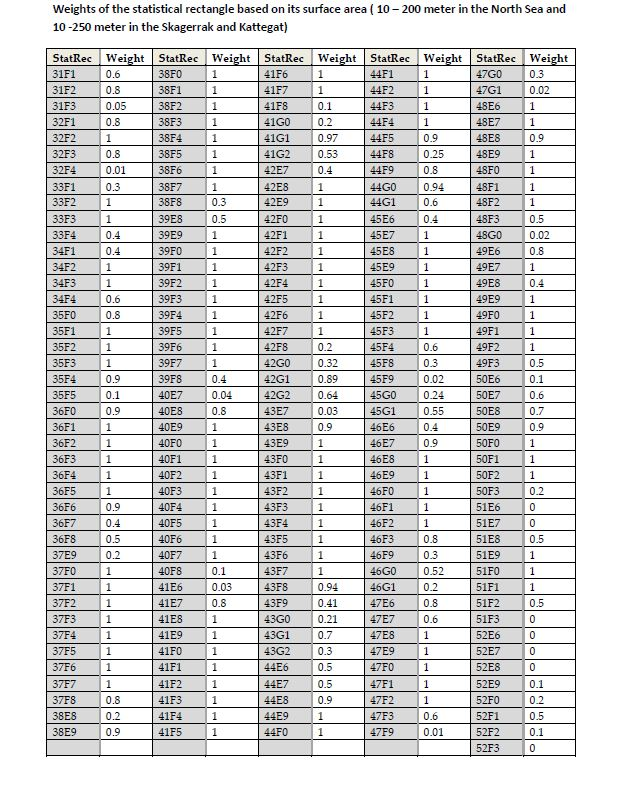
\includegraphics[width=10.5cm]{recWeightings.jpg}}   
 \captionsetup{font= footnotesize, width=15cm}{
 \caption{}\label{weightings11}}
\end{figure}
 
\end{appendices}



\end{document}